%%%%%%%%%%%%%%%%%
%               %
%   SETUP       %
%               %
%%%%%%%%%%%%%%%%%
\documentclass[english, version-2019-07]{uzl-thesis}
\UzLStyle{computer modern oldschool design}
\UzLThesisSetup{
  Masterarbeit,
  Titel auf Deutsch     = {Identification genetischer Risikovarianten für Artheriosklerose via oxidativem Stress Assay in glatten Muskulaturzellen und bioinformatische Ansätze},
  Titel auf Englisch    = {Identification of genetic risk variants for atherosclerosis using oxidative stress assays in vascular smooth muscle cells and bioinformatic approaches
},
  Logo-Dateiname        = {Logo_Inst_Kardiogenetik_RGB.JPG},
  Verfasst              = {am}{Institut für Kardiogenetik},
  Autor                 = {Torben Falk},
  Betreuerin            = {Prof. Dr. Jeanette Erdmann},
  Mit Unterstützung von = {Dr. Tobias Reinberger},
  Studiengang           = {Molecular Life Science},
  Datum                 = {26. Juli 2022},
  Zusammenfassung       = {
    {\Large ÜBERETZTEN}

“Cardiovascular diseases (CVD) are the leading cause of death globally, taking an estimated 17.9 million lives each year.”, according to the world health organization (WHO) \cite{whoCardiovascularDiseases2022}. The most common CVD is coronary artery disease (CAD) \cite{centersfordiseasecontrolandpreventionHeartDiseaseFacts2022}, which poses a significant challenges for current and future medical professionals. Investigating the molecular basics of this pathological process is pivotal for developing suitable treatment options.
While vascular smooth muscle cells (VSMC) are essential in initiating and maintaining atherosclerotic plaques \cite{doranRoleSmoothMuscle2008}, the exact model for their exact role and function is frequently updated \cite{liuSmoothMuscleCell2019, grootaertVascularSmoothMuscle2021, yapSixShadesVascular2021}. We hypothesize that extensive stimulation of VSMCs with pro-inflammatory cytokines such as PDGF-BB can cause oxidative stress and promote disease progression.
For this, we recapitulated that PDGF-BB boost of in vitro dedifferentiated HAoSMCs induces the generation of reactive oxygen species (ROS). Further, we tested the limits of the CellROX\texttrademark Assay to evaluate this interaction. We conclude that the assay provides a solid basis for the analysis of ROS generation due to PDGF-BB stimulation. Additionally, we suggest optimizations to the assay to improve its reproducibility.
In contrast to this hypothesis-driven approach, GWA studies are a tremendous observational tool for identifying exciting research targets \cite{uffelmannGenomewideAssociationStudies2021}.
To complement CAD GWA study data, we curated and funneled genomic annotations of regulatory elements into a database. This database serves as the foundation of the GWAS Navigator. The GWAS Navigator is an interactive web-based visualization tool. It provides easy access to CAD GWA study summary statistics and their genomic context.
Finally, we integrated the curated data in an enrichment analysis. Testing for overlap of CAD risk variants with tissue- and cell-specific regulatory elements. We found overrepresentation of overlaps mainly in biosamples from the heart, arteries, or lungs — a result that underlines the frequently described connection between heart- and lung diseases \cite{carterAssociationCardiovascularDisease2019, nowakLungFunctionCoronary2018, hanPulmonaryDiseasesHeart2007}.

  },
  Abstract              = {
    “\Acp{cvd} are the leading cause of death globally, taking an estimated 17.9 million lives each year.”, according to the \ac{who} \cite{whoCardiovascularDiseases2022}. The most common CVD is \ac{cad} \cite{centersfordiseasecontrolandpreventionHeartDiseaseFacts2022}, which poses a significant challenge for current and future medical professionals. Investigating the molecular basics of this pathological process is pivotal for developing suitable treatment options.\\
While \acp{vsmc} are essential in initiating and maintaining atherosclerotic plaques \cite{doranRoleSmoothMuscle2008}, the exact model for their precise role and function is frequently updated \cite{liuSmoothMuscleCell2019, grootaertVascularSmoothMuscle2021, yapSixShadesVascular2021}. We hypothesize that extensive stimulation of \acp{vsmc} with pro-inflammatory cytokines such as ac{pdgf} can cause oxidative stress and promote disease progression.\\
For this, we recapitulated that \acs{pdgf} boost of in vitro dedifferentiated \ac{haosmc} induces the generation of \ac{ros}. Further, we tested the limits of the CellROX\texttrademark Assay to evaluate this interaction. We conclude that the assay provides a solid basis for analyzing \ac{ros} generation due to \ac{pdgf} stimulation. Additionally, we suggest optimizations to the assay to improve its reproducibility.\\
In contrast to this hypothesis-driven approach, \acp{gwas} are a tremendous observational tool for identifying exciting research targets \cite{uffelmannGenomewideAssociationStudies2021}. To complement \ac{cad} \ac{gwas} data, we curated and funneled genomic annotations of regulatory elements into a database. This database serves as the foundation of the \aca{gwas} Navigator, an interactive web-based visualization tool. It provides easy access to \ac{cad} \aca{gwas} GWA study summary statistics and their genomic context.\\
Finally, we integrated the curated data into an enrichment analysis — testing for overlap of \ac{cad} risk variants with tissue- and cell-specific regulatory elements. We found an overrepresentation of overlaps mainly in biosamples from the heart, arteries, or lungs — a result that underlines the frequently described connection between heart- and lung diseases \cite{carterAssociationCardiovascularDisease2019, nowakLungFunctionCoronary2018, hanPulmonaryDiseasesHeart2007}.

  },
  % Alphabetische Bibliographie,
  % Numerische Bibliographie,
  Acknowledgements = {
  First and foremost, I'd like to thank Dr. Tobias Reinberger for his outstanding supervision. Thank you for always making time for my questions, great advice, motivating words, and genuine interest in my project. Further, I'd like to thank Prof. Dr. Jeanette Erdmann for giving me the chance to be a part of her lab and for her excellent feedback - I truly learned a lot! I'd like to thank Lisa Diner for taking care of my cells when I wasn't available and answering my frequent questions. Of course, I'd like to thank all the other group members. Thank you for the welcoming atmosphere, delicious cake, necessary breaks, and excellent scientific advice!\\
  In addition, this thesis marks the end of my studies at the University of Lübeck. I'd like to thank all the friends who supported me during this time. Those who are becoming incredible scientists themselves and those who enrich my life by having totally different interests. I value your opinions very much, and thank you for taking my mind off my studies sometimes. I appreciate every single one of you; you made Lübeck feel like home.\\
  Finally, I'd like to thank my parents for their immense support. I love you.
  }
}

\usepackage[
style=authoryear,
maxcitenames=2,
dashed=false,
uniquename=init,
backend=bibtex,
sorting=none,
url=false,
doi=true,
isbn=false,
date=year
]{biblatex}

%
% Till Tantau's code for reproducing the Cell bibliography style
% in biblatex:
%
\DeclareNameAlias{sortname}{last-first}
\setlength{\bibhang}{0pt}
\setlength{\bibitemsep}{1em}
\renewcommand*{\bibinitdelim}{}
\renewbibmacro*{in:}{%
  \iffieldequalstr{entrytype}{inproceedings}{%
    \printtext{\bibstring{in}\addspace}%
  }{}%
}
\DeclareFieldFormat[book]{title}{##1\isdot}
\DeclareFieldFormat[inproceedings]{title}{##1\isdot}
\DeclareFieldFormat{booktitle}{##1\addcomma}
\renewbibmacro*{byeditor+others}{%
  \ifnameundef{editor}
  {}
  {\printtext[parens]{%
      \printnames[paren]{editor}%
      \addcomma\addspace
      \usebibmacro{editorstrg}%
    }
    \setunit{\addspace}
    \newunit}%
  \usebibmacro{byeditorx}%
  \usebibmacro{bytranslator+others}}
%
\DeclareFieldFormat[article,inbook,incollection,inproceedings,patent,thesis,unpublished]{title}{##1}
\DeclareFieldFormat[article]{journaltitle}{##1\isdot}
\DeclareFieldFormat[article]{volume}{\textit{##1}}
\DeclareFieldFormat[article]{pages}{##1}
\renewbibmacro*{volume+number+eid}{\printfield{volume}}
\renewcommand*{\nameyeardelim}{\addcomma\addspace}
\DeclareCiteCommand{\cite}[\mkbibparens]
  {\usebibmacro{prenote}}
  {\usebibmacro{citeindex}%
    \usebibmacro{cite}}
  {\multicitedelim}
  {\usebibmacro{postnote}}
\DeclareCiteCommand*{\cite}[\mkbibparens]
  {\usebibmacro{prenote}}
  {\usebibmacro{citeindex}%
    \usebibmacro{citeyear}}
  {\multicitedelim}
  {\usebibmacro{postnote}}


% Changes in Article
\DeclareFieldFormat[article]{title}{#1}
\DeclareFieldFormat[article]{journaltitle}{#1\isdot}
\DeclareFieldFormat[article]{volume}{\textit{#1}}
\DeclareFieldFormat[article]{pages}{#1}

\addbibresource{Literatur/literatur.bib}

\AtEveryBibitem{\clearfield{note}}
\AtEveryCitekey{\clearfield{note}}

\AtEveryBibitem{\clearfield{abstract}}
\AtEveryCitekey{\clearfield{abstract}}

\AtEveryBibitem{\clearfield{eprint}}
\AtEveryCitekey{\clearfield{eprint}}

\AtEveryBibitem{\clearfield{eprinttype}}
\AtEveryCitekey{\clearfield{eprinttype}}

%Packages
\usepackage{lscape}
\usepackage{tabularx}
\usepackage{tabularray}
\usepackage{textgreek}
\usepackage{siunitx}
\usepackage{multirow}
\usepackage{enumerate}
%\usepackage[printonlyused]{acronym}
\usepackage[flushleft]{threeparttable}
\usepackage{layouts}
\usepackage{hypcap}
\usepackage[super]{nth}
\usepackage{float}

\usepackage{acro}
\usepackage{pdfcomment}
\acsetup{
  pdfcomments/use=true
}
\DeclareAcronym{24 well}{
short = 24-well multidish,
short-plural-form = 24-well multidishes,
long = Nunc\texttrademark Cell-Culture Treated Multidish 24,
pdfcomment = Nunc\texttrademark Cell-Culture Treated Multidish 24,
tag = acronym}

\DeclareAcronym{abc}{
short = ABC,
long = activity by contact,
pdfcomment = activity by contact,
tag = acronym}

\DeclareAcronym{api}{
short = API,
long = application programming interface,
pdfcomment = application programming interface,
tag = acronym}

\DeclareAcronym{atac}{
short = ATAC-seq,
long = assay for transposase-accessible chromatin using sequencing,
pdfcomment = assay for transposase-accessible chromatin using sequencing,
tag = acronym}

\DeclareAcronym{atp}{
short = ATP,
long = adenosine triphosphate,
pdfcomment = adenosine triphosphate,
tag = acronym}

\DeclareAcronym{cad}{
short = CAD,
long = coronary artery disease,
pdfcomment = coronary artery disease,
tag = acronym}

\DeclareAcronym{camp}{
short = cAMP,
long = cyclic adenosine monophosphate,
pdfcomment = cyclic adenosine monophosphate,
tag = acronym}

\DeclareAcronym{cCRE}{
short = cCRE,
long = candidate cis-regulatory element,
pdfcomment = candidate cis-regulatroy element,
tag = acronym}

\DeclareAcronym{cnn1}{
short = CNN1,
long = calponin 1,
pdfcomment = calponin 1,
tag = acronym}

\DeclareAcronym{co2}{
short = CO\textsubscript{2},
long = carbon dioxide,
pdfcomment = carbon dioxide,
tag = acronym}

\DeclareAcronym{col1}{
short = Col I,
long = collagen type I,
pdfcomment = collagen type I,
tag = acronym}

\DeclareAcronym{copd}{
short = COPD,
long = chronic obstructive pulmonary disease,
pdfcomment = chronic obstructive pulmonary disease,
tag = acronym}

\DeclareAcronym{Cq}{
short = Cq,
long = quantification cycle,
pdfcomment = quantification cycle,
tag = acronym}

\DeclareAcronym{crispr}{
short = CRISPR,
long = clustered regularly interspaced short palindromic repeats,
pdfcomment = clustered regularly interspaced short palindromic repeats,
tag = acronym}

\DeclareAcronym{css}{
short = CSS,
long = cascading style sheets,
pdfcomment = cascading style sheets,
tag = acronym}

\DeclareAcronym{ctcf}{
short = CTCF,
long = CCCTC binding factor,
pdfcomment = CCCTC binding factor,
tag = acronym}

\DeclareAcronym{d}{
short = d,
long = day(s),
pdfcomment = day(s),
tag = unit}

\DeclareAcronym{de}{
short = DE,
long = Deutschland,
pdfcomment = Deutschland,
tag = country}

\DeclareAcronym{dELS}{
short = dELS,
long = distal enhancer-like elements,
sort = ELS,
pdfcomment = distal enhancer-like elements,
tag = acronym}

\DeclareAcronym{dna}{
short = DNA,
long = deoxyribonucleic acid,
pdfcomment = deoxyribonucleic acid,
tag = acronym}

\DeclareAcronym{dNTP}{
short = dNTP,
long = deoxyribose nucleoside triphosphate,
pdfcomment = deoxyribose nucleoside triphosphate,
tag = acronym}

\DeclareAcronym{dock2}{
short = Dock2,
long = dedicator of cytokinesis 2,
pdfcomment = dedicator of cytokinesis 2,
tag = acronym}

\DeclareAcronym{DTT}{
short = DTT,
long = reverse transcription,
pdfcomment = reverse transcription,
tag = acronym}

\DeclareAcronym{ec50}{
short = EC\textsubscript{50},
long = half maximal effective concentration,
pdfcomment = half maximal effective concentration,
tag = acronym}

\DeclareAcronym{ecar}{
short = ECAR,
long = extracellular acidification rate,
pdfcomment = extracellular acidification rate,
tag = acronym}

\DeclareAcronym{ecm}{
short = ECM,
long = extracellular matrix,
pdfcomment = extracellular matrix,
tag = acronym}

\DeclareAcronym{elk-1}{
short = Elk-1,
long = ETS like-1 protein,
pdfcomment = ETS like-1 protein,
tag = acronym}

\DeclareAcronym{encode}{
short = ENCODE,
long = ENCyclopedia Of DNA Elements project,
pdfcomment = ENCyclopedia Of DNA Elements project,
tag = acronym}

\DeclareAcronym{eqtl}{
short = eQTL,
long = expression quantitative trait loci,
pdfcomment = expression quantitative trait loci,
tag = acronym}

\DeclareAcronym{er}{
short = ER,
long = entity-relationship,
pdfcomment = entity-relationship,
tag = acronym}

\DeclareAcronym{fbs}{
short = FBS,
long = fetal bovine serum,
pdfcomment = fetal bovine serum,
tag = acronym}

\DeclareAcronym{fccp}{
short = FCCP,
long = carbonyl cyanide-p-trifluoromethoxyphenylhydrazone,
pdfcomment = carbonyl cyanide-p-trifluoromethoxyphenylhydrazone,
tag = acronym}

\DeclareAcronym{fev1}{
short = FEV\textsubscript{1},
long = forced expiratory volume in 1 second,
pdfcomment = forced expiratory volume in 1 second,
tag = acronym}

\DeclareAcronym{ftp}{
short = FTP,
long = file transfer protocol,
pdfcomment = file transfer protocol,
tag = acronym}

\DeclareAcronym{gapdh}{
short = GAPDH,
long = glyceraldehyde-3-phosphate dehydrogenase,
pdfcomment = glyceraldehyde-3-phosphate dehydrogenase,
tag = acronym}

\DeclareAcronym{gsea}{
short = GES analysis,
short-plural-form = GES analyses,
long = gene set enrichment analysis,
long-plural = gene set enrichment analyses,
pdfcomment = gene set enrichment analysis,
tag = acronym}

\DeclareAcronym{gi}{
short = GI,
long = gastrointestinal,
pdfcomment = gastrointestinal,
tag = acronym}

\DeclareAcronym{gwas}{
short = GWA study,
alt = GWAS,
alt-plural-form = GWAS,
long = genome wide association study,
short-plural-form = GWA studies,
long-plural-form = genome wide association studies,
pdfcomment = genome wide association study,
tag = acronym}

\DeclareAcronym{h}{
short = h,
long = hour(s),
pdfcomment = hour(s),
tag = unit}

\DeclareAcronym{H3K27ac}{
short = H3K27ac,
long = histone 3 lysine 27 acetylation,
pdfcomment = histone 3 lysine 27 acetylation,
tag = acronym}

\DeclareAcronym{H3K4me3}{
short = H3K4me3,
long = histone 3 lysine 4 trimethylation,
pdfcomment = histone 3 lysine 4 trimethylation,
tag = acronym}

\DeclareAcronym{h2o2}{
short = H\textsubscript{2}O\textsubscript{2},
long = hydrogen peroxide,
pdfcomment = hydrogen peroxide,
tag = acronym}

\DeclareAcronym{haosmc}{
short = HAoSMC,
long = human aortic \ac{smc},
pdfcomment = human aortic \ac{smc},
tag = acronym}

\DeclareAcronym{hbss}{
short = HBSS,
long = Hanks balanced salt solution,
pdfcomment = Hanks balanced salt solution,
tag = acronym}

\DeclareAcronym{hf}{
short = HF,
long = heart failure,
pdfcomment = heart failure,
tag = acronym}

\DeclareAcronym{hg19}{
short = hg19,
long = Genome Reference Consortium Human Build 37,
pdfcomment = Genome Reference Consortium Human Build 37,
tag = acronym}

\DeclareAcronym{hg38}{
short = hg38,
long = Genome Reference Consortium Human Build 38,
pdfcomment = Genome Reference Consortium Human Build 38,
tag = acronym}

\DeclareAcronym{hgnc}{
short = HGNC,
long = Human Gene Nomenclature Consortium,
pdfcomment = Human Gene Nomenclature Consortium,
tag = acronym}

\DeclareAcronym{html}{
short = HTML,
long = hypertext markup language,
pdfcomment = hypertext markup language,
tag = acronym}

\DeclareAcronym{ifn}{
short = IFN,
long = interferon,
pdfcomment = interferon,
tag = acronym}

\DeclareAcronym{il1}{
short = IL-1\beta,
long = interleukin 1 beta,
pdfcomment = interleukin 1 beta,
tag = acronym}

\DeclareAcronym{js}{
short = JS,
long = javascript,
pdfcomment = javascript,
tag = acronym}

\DeclareAcronym{json}{
short = JSON,
long = JavaScript Object Notation,
pdfcomment = JavaScript Object Notation,
tag = acronym}

\DeclareAcronym{klf4}{
short = KLF4,
long = Kruppel-like factor 4,
pdfcomment = Kruppel-like factor 4,
tag = acronym}

\DeclareAcronym{l2g}{
short = L2G,
long = link to gene,
pdfcomment = link to gene,
tag = acronym}

\DeclareAcronym{ld}{
short = LD,
long = linkage disequilibrium,
pdfcomment = linkage disequilibrium,
tag = acronym}

\DeclareAcronym{M231}{
short = M231,
long = Human Vascular Smooth Muscle Cell Basal Medium (Medium 231),
pdfcomment = Human Vascular Smooth Muscle Cell Basal Medium (Medium 231),
tag = acronym}

\DeclareAcronym{maf}{
short = MAF,
long = minor allele frequency,
pdfcomment = minor allele frequency,
tag = acronym}

\DeclareAcronym{map}{
short = MAP,
long = mitogen activated protein,
pdfcomment = mitogen activated protein,
tag = acronym}

\DeclareAcronym{mi}{
short = MI,
long = myocardial infarction,
pdfcomment = myocardial infarction,
tag = acronym}

\DeclareAcronym{min}{
short = min,
long = minute(s),
pdfcomment = minute(s),
tag = unit}

\DeclareAcronym{mmp}{
short = MMP,
long = matrix metallopeptidase,
pdfcomment = matrix metallopeptidase,
tag = acronym}

\DeclareAcronym{mmp9}{
short = MMP9,
long = \ac{mmp} 9,
pdfcomment = matrix metallopeptidase 9,
tag = acronym}

\DeclareAcronym{nac}{
short = NAC,
long = N-acetylcysteine,
pdfcomment = N-acetylcysteine,
tag = acronym}

\DeclareAcronym{o2}{
short = O\textsubscript{2},
long = elemental oxygen,
pdfcomment = elemental oxygen,
tag = acronym}

\DeclareAcronym{o2-}{
short = O\textsubscript{2}\textsuperscript{•-},
short-plural-form = O\textsubscript{2}\textsuperscript{•-},
long = superoxide anion radical,
pdfcomment = superoxide anion radical,
tag = acronym}

\DeclareAcronym{ocr}{
short = OCR,
long = oxygen consumption rate,
pdfcomment = oxygen consumption rate,
tag = acronym}

\DeclareAcronym{pbs}{
short = PBS,
long = phosphate buffered solution,
pdfcomment = phosphate buffered solution,
tag = acronym}

\DeclareAcronym{pcr}{
short = PCR,
long = polymerase chain reaction,
pdfcomment = polymerase chain reaction,
tag = acronym}

\DeclareAcronym{pdgf_simple}{
short = PDGF,
long = platelet-derived growth factor,
pdfcomment = platelet-derived growth,
tag = acronym}

\DeclareAcronym{pdgf}{
short = PDGF-BB,
long = \ac{pdgf_simple}-BB,
pdfcomment = platelet-derived growth factor-BB,
tag = acronym}

\DeclareAcronym{pdgfr}{
short = PDGFR,
long = \ac{pdgf_simple} receptor,
pdfcomment = platelet-derived growth factor receptor,
tag = acronym}

\DeclareAcronym{pELS}{
short = pELS,
sort = ELS,
long = proximal enhancer-like elements,
pdfcomment = proximal enhancer-like elements,
tag = acronym}

\DeclareAcronym{PI3K}{
short = PI3K,
long = phosphatidylinositol 3'-kinase,
pdfcomment = phosphatidylinositol 3'-kinase,
tag = acronym}

\DeclareAcronym{pip}{
short = PIP,
long = posterior inclusion probability,
long-plural-form = posterior inclusion probabilities,
pdfcomment = posterior inclusion probability,
tag = acronym}

\DeclareAcronym{PLS}{
short = PLS,
long = promoter-like elements,
pdfcomment = promoter-like elements,
tag = acronym}

\DeclareAcronym{qpcr}{
short = qPCR,
long = quantitative \ac{pcr},
sort = PCR,
pdfcomment = quantitative \ac{pcr},
tag = acronym}

\DeclareAcronym{rest}{
short = REST,
long = representational state transfer,
pdfcomment = representational state transfer,
tag = acronym}

\DeclareAcronym{rna}{
short = RNA,
long = ribonucleic acid,
pdfcomment = ribonucleic acid,
tag = acronym}

\DeclareAcronym{ros}{
short = ROS,
long = reactive oxygen species,
pdfcomment = reactive oxygen species,
tag = acronym}

\DeclareAcronym{RT}{
short = RT,
long = reverse transcription,
pdfcomment = reverse transcription,
tag = acronym}

\DeclareAcronym{sc}{
short = sc,
long = single-cell,
pdfcomment = single-cell,
tag = acronym}

\DeclareAcronym{sca1}{
short = Sca1,
long = stem cell antigen-1,
pdfcomment = stem cell antigen-1,
tag = acronym}

\DeclareAcronym{smgs}{
short = SMGS,
long = Smooth Muscle Cell Growth Supplement,
pdfcomment = Smooth Muscle Cell Growth Supplement,
tag = acronym}

\DeclareAcronym{snp}{
short = SNP,
long = single nucleotide polymorphism,
pdfcomment = single nucleotide polymorphism,
tag = acronym}

\DeclareAcronym{sp1}{
short = Sp1,
long = specificity protein 1,
pdfcomment = specificity protein 1,
tag = acronym}

\DeclareAcronym{sql}{
short = SQL,
long = structured query language,
pdfcomment = structured query language,
tag = acronym}

\DeclareAcronym{srf}{
short = SRF,
long = serum response factor,
pdfcomment = serum response factor,
tag = acronym}

\DeclareAcronym{stat}{
short = STAT,
long = signal transducers and activators of transcription,
pdfcomment = signal transducers and activators of transcription,
tag = acronym}

\DeclareAcronym{stat1}{
short = STAT1,
long = \ac{stat}1,
pdfcomment = \ac{stat}1,
tag = acronym}

\DeclareAcronym{tad}{
short = TAD,
long = topologically associated domain,
pdfcomment = topologically associated domain,
tag = acronym}

\DeclareAcronym{tf}{
short = TF,
long = transcription factor,
pdfcomment = transcription factor,
tag = acronym}

\DeclareAcronym{tgf}{
short = TGF\beta,
long = Transforming Growth Factor beta,
pdfcomment = transforming Growth Factor beta,
tag = acronym}

\DeclareAcronym{tss}{
short = TSS,
long = transcription start sites,
pdfcomment = transcription start sites,
tag = acronym}

\DeclareAcronym{USCS}{
short = USCS,
long = University of California Santa Cruz,
pdfcomment = University of California Santa Cruz,
tag = acronym}

\DeclareAcronym{vep}{
short = VEP,
long = variant effect predictor,
pdfcomment = variant effect predictor,
tag = acronym}

\DeclareAcronym{vsmc}{
short = vSMC,
long = vascular \ac{smc},
sort = smooth muscle cell,
pdfcomment = vascular \ac{smc},
tag = acronym}

\DeclareAcronym{smc}{
short = SMC,
long = smooth muscle cell,
pdfcomment = smooth muscle cell,
tag = acronym}

\DeclareAcronym{wgs}{
short = WGS,
long = whole genome sequencing,
pdfcomment = whole genome sequencing,
tag = acronym}

\DeclareAcronym{mRNA}{
short = mRNA,
sort = RNA,
long = messenger-\ac{rna},
pdfcomment = messenger-\ac{rna},
tag = acronym}

\DeclareAcronym{lncRNA}{
short = lncRNA,
long = long non-coding \ac{rna},
sort = RNA,
pdfcomment = long non-coding \ac{rna},
tag = acronym}

\DeclareAcronym{miRNA}{
short = miRNA,
long = micro \ac{rna},
sort = RNA,
pdfcomment = micro \ac{rna},
tag = acronym}

\DeclareAcronym{cDNA}{
short = cDNA,
long = complementary  \ac{dna},
sort = DNA,
pdfcomment = complementary  \ac{dna},
tag = acronym}

\DeclareAcronym{celsius}{
short = °C,
long = degree celsius,
tag = unit}

\DeclareAcronym{s}{
short = s,
long = second(s),
tag = unit}

\DeclareAcronym{mL}{
short = mL,
long = milliliter,
tag = unit}

\DeclareAcronym{µL}{
short = µL,
long = microliter,
tag = unit}

\DeclareAcronym{pM}{
short = pM,
long = picomolar,
tag = unit}

\DeclareAcronym{nM}{
short = nM,
long = nanomolar,
tag = unit}

\DeclareAcronym{µM}{
short = µM,
long = micromolar,
tag = unit}

\DeclareAcronym{mM}{
short = mM,
long = milimolar,
tag = unit}

\DeclareAcronym{M}{
short = M,
long = molar,
tag = unit}

\DeclareAcronym{µg}{
short = µg,
long = microgram,
tag = unit}

\DeclareAcronym{mg}{
short = mg,
long = milligram,
tag = unit}

\DeclareAcronym{water}{
short = H\textsubscript{2}0,
long = dihydrogen monoxide (water),
tag = acronym}

\DeclareAcronym{dapi}{
short = DAPI,
long = {4',6-diamidino-2-phenylindole},
tag = acronym}

\DeclareAcronym{if}{
short =IF,
long = immunofluorescence,
tag = acronym}

\DeclareAcronym{ef}{
short =ef,
long = enrichment factor,
tag = acronym}

\DeclareAcronym{bsa}{
short =BSA,
long = bovine serum albumin,
tag = acronym}

\DeclareAcronym{cvd}{
short =CVD,
long = cardiovascular disease,
tag = acronym}

\DeclareAcronym{who}{
short =WHO,
long = world health organization,
tag = acronym}


%Grafiken
\graphicspath{{C:/Users/torbe/OneDrive/Dokumente/Uni/Masterarbeit/Thesis/Abbildung/}}

%Hersteller:

\newcommand{\Roth}{Carl Roth GmbH + Co. KG}
\newcommand{\SigmaA}{Sigma-Aldrich Co. LLC.}
\newcommand{\Merck}{Merck KGaA}
\newcommand{\Thermo}{Thermo Fisher Scientific Inc.}
\newcommand{\Sarstedt}{Sarstedt AG \& Co.}
\newcommand{\Eppendorf}{Eppendorf SE}
\newcommand{\Brand}{Brand GmbH \& Co. KG}
\newcommand{\PeproTech}{PeproTech\copyright}
\newcommand{\Invitrogen}{Invitrogen\texttrademark AG}
\newcommand{\NEB}{New England Biolabs GmbH}
\newcommand{\Baker}{J.T.Baker\textregistered}
\newcommand{\Keyence}{Keyence Corporation}
\newcommand{\Agilent}{Agilent Technologies, Inc.}
\newcommand{\LifeTech}{Life Technologies Limited}
\newcommand{\AB}{Applied Biosystems}
\newcommand{\Lonza}{Lonza Group AG}
\newcommand{\Ibidi}{ibidi GmbH}
\newcommand{\Biosell}{Bio\&SELL GmbH}
\newcommand{\Assistent}{Glaswarenfabrik Karl Hecht GmbH \& Co. KG}
\newcommand{\Kisker}{Kisker Biotech GmbH \& Co. KG}
\newcommand{\chemometec}{ChemoMetec A/S}
\newcommand{\Pechiney}{Pechiney Plastic Packaging, Inc.}
\newcommand{\Sartorius}{Sartorius AG}
\newcommand{\Heidolph}{Heidolph Instruments Labortechnik}
\newcommand{\SensoQuest}{SensoQuest GmbH}
\newcommand{\Hettich}{Andreas Hettich GmbH \& Co. KG}
\newcommand{\Heraeus}{Heraeus Holding GmbH}
\newcommand{\Gibco}{Gibco\textregistered BRL}
\newcommand{\Nikon}{Nikon Corporation}

%Farben
\definecolor{mygray}{gray}{0.5}
\definecolor{myblue}{RGB}{74,134,232}
\definecolor{mygreen}{RGB}{0,0,0}
\definecolor{myred}{RGB}{152,0,0}
\definecolor{myyellow}{RGB}{255,153,0}
\definecolor{external_link}{RGB}{51,102,187}
\definecolor{internal_link}{RGB}{6,69,173}

\hypersetup{
	colorlinks   = true,
	urlcolor  = external_link,
  	citecolor = internal_link
}

%commands
\newcommand\TILDE{\char`\~}
\newlength{\captionwidth}
\setlength{\captionwidth}{0.9\textwidth}
\newcommand{\MYhref}[2]{\href{#1}{\color{myblue}{#2}}}

%%%%%%%%%%%%%%%%%
%               %
%  START OF DOC %
%               %
%%%%%%%%%%%%%%%%%

\begin{document}
\fontdimen16\textfont2=3pt
\fontdimen17\textfont2=3pt

\DefTblrTemplate{caption-tag}{default}{}
\DefTblrTemplate{caption-sep}{default}{}
\DefTblrTemplate{caption-text}{default}{}

\acuse{rna, dna, h, min, d, s, celsius, mL, µL, pM, nM, µM, mM, M, µg, mg, water, 24 well, bsa}


%%%%%%%%%%%%%%%%%
%               %
%   Grundlagen  %
%               %
%%%%%%%%%%%%%%%%%

\chapter{Introduction}
\section{Coronary artery disease}
\label{sec:cad}
- CAD is serious.
- Describe the pheontype
- Describe prevalence
- Check intro of Anja, papers for more info
- Go into treatment and Risk
- herditary parts in disease

\section{GWAS}
\label{sec:gwas}

    \subsection{GWAS}
    \label{subsec:gwas_general}
    What are GWAS. Describe how it works, why we do it.

    \subsection{Post GWAS}
    \label{subsec:gwas_limit}
    And their limitations. Possible follow up studies. Focus on computational and cell based assays.

\section{Muscle Cells in CAD}
\label{sec:haosms}
- We now that smooth muscle cells play a key role
- It is widely accepted that there is not only one type of smooth muscle cell
- Go into the contractile phenotype and synthetic phenotype
    - TGFb or PDGF used to induce them
    - contractile phenotype is thought to be protective

\section{PDGF Signaling and Oxidative Stress}
\label{sec:haosms}
    \subsection{PDGF Signaling}
    \label{subsec:pdf_signaling}

    \subsection{ROS}
    \label{subsec:ROS}
    - ROS in general and the role of ROS in disease

    \subsection{ROS in PDGF Signaling}
    \label{subsec:ROS_signaling}
    - ROS as a second messenger in PDGF signaling

\section{Complementary High Through Put Methods}
\label{sec:bioinformatics}

    \subsection{Linkage Disequilibrium}
    Linkage disequilibrium is a parameter from populations genetics that describes the non-random association of two or more allels. The LD is often quantified using the correlation coefficient $r^2$ \cite{slatkinLinkageDisequilibriumUnderstanding2008}.

    $$ D_{AB} = p_{AB} − p_A p_B $$
    $$ r^2 = \frac{D_{AB}^2}{p_A (1-p_A) \times p_B (1-p_B)} $$

    Where $pA$ and $pB$ is the frequency of the alleles A and B respectively. $pAB$ is the frequency of the AB haplotype.

    \subsection{Locus To Gene Scores}

    \subsection{Regulatory Build}
    The ensembl regulatory build compiles a summary of regulatory regions found in the human genome. It is build on the basis publically available epigenetic marks and transcription factor binding and contains Promotors, Proximal enhancers, distal enhancers and CTCF binding sites \cite{zerbinoEnsemblRegulatoryBuild2015}.

    \subsection{ENCODE cCREs}

    \subsection{scATAC Seq}

    \subsection{ABC Model}

    \subsection{TADs}

\section{Aim of the thesis}
\label{sec:Aim}
- Build tool for visual exploration of the CAD GWAS data.
- Establish a system to test the role of ROS in CAD.


%%%%%%%%%%%%%%%%%
%               %
%   Material    %
%               %
%%%%%%%%%%%%%%%%%

\chapter{Material}

\section{Manufactors}
\label{sec:manufactors}
\begin{longtblr}[]{
    colspec = {X|X},
    rowhead = 1
}
    \textbf{Manufacturer} & \textbf{Seat}\\ \hline
    \Agilent  & Santa Clara, CA, USA\\
    \Assistent & Sondheim vor der Rhön, DE\\
    \Brand & Wertheim, DE\\
    \chemometec & Allerod, DK \\
    \Eppendorf & Hamburg, DE\\
    \Heraeus & Hanau, DE \\
    \Merck & Darmstadt, DE \\
    \Keyence & Osaka, JP\\
    \Kisker & Steinfurt, DE \\
    \Sarstedt & Nürnberg, DE \\
    \SigmaA & St. Louis, MO, USA\\
    \Thermo & Waltham, MA, USA \\
    \PeproTech \newline (Brand of \Thermo) & Hamburg, DE \\
    \Pechiney & Chicago, IL, USA \\
    \Baker \newline (Brand of \Thermo) & Schwerte, DE \\
    GFL mbH & Burgwedel, DE \\
    \AB \newline (Brand of LUMITOS AG) & Warrington, UK\\
    \Gibco \newline (Brand of \Thermo) & Gaithersburg, MD, USA \\
    \Ibidi & Gräfelfing, DE\\
    \Invitrogen \newline (Brand of \Thermo)& Schwerte, DE\\
    \Lonza & Basel, CHE \\
    \Biosell & Feucht, DE\\
    \NEB & Ipswich, MA, USA \\
    \Nikon & Minato, JP\\
    \Sartorius & Göttingen, DE \\
    \SensoQuest & Göttingen, DE \\
    Hanna Instruments Deutschland GmbH & Vöhringen, DE \\
    \Heidolph & Schwabach, DE\\
    ZIEGRA Eismaschinen GmbH & Isernhagen, DE \\
    Mettler-Toledo GmbH & Gießen, DE \\
    Serif (Europe) Ltd. & Nottingham, UK\\
    Microsoft Deutschland GmbH  & München, DE\\
    GitHub, Inc. \newline (Part of Microsoft Corporation)  & San Francisco, CA, USA \\
    Python Software Foundation  & Beaverton, OR, USA\\
    JetBrains s.r.o.  & Prague, CZ\\
    The SQLite Consortium \newline (Contact via Hipp, Wyrick \& Company) & Charlotte, NC, USA\\
\end{longtblr}



\section{Celllines}
\label{sec:cells}
\begin{longtblr}[]{
    colspec = {X|X|X},
    rowhead = 1
}
    \textbf{Name}                            & \textbf{Celltype}    & \textbf{Manufacturer} \\ \hline
    Human Aortic Smooth Muscle Cell (HAoSMC) & prim. human cell     & \textbf{\color{red} ?!?}             \\
\end{longtblr}

\section{Primer}
\label{sec:primer}
\begin{longtblr}[]{
    colspec = {X|X|X[3]},
    rowhead = 1
}
\textbf{Target}                 & \textbf{Name}  & \textbf{Sequence}  \\ \hline
\SetCell[r=2]{m}CNN1            & Fw   & \textbf{\color{red} 5'-seq-3'} \\
                                & Rv   & \textbf{\color{red} 5'-seq-3'} \\
\SetCell[r=2]{m}GAPDH           & Fw   & \textbf{\color{red} 5'-seq-3'} \\
                                & Rv   & \textbf{\color{red} 5'-seq-3'} \\
\SetCell[r=2]{m}MMP9            & Fw   & \textbf{\color{red} 5'-seq-3'} \\
                                & Rv   & \textbf{\color{red} 5'-seq-3'} \\
\end{longtblr}

\section{Chemicals}
\label{sec:chemicals}
\begin{longtblr}[]{
    colspec = {X|X},
    rowhead = 1
}
    \textbf{Name} &  \textbf{Manufacturer} \\ \hline
    5X First Strand Buffer & \Invitrogen \\
    Antimycin A & \SigmaA \\
    BSA & \textbf{\color{red} ?!?} \\
    CellROX\texttrademark Green Reagent & \Thermo \\
    Collagen Type I, rat tail & \Ibidi \\
    dNTP Mix & \AB \\
    DTT & \Invitrogen \\
    Ethanol (99.9 \%) & \Baker \\
    \acs{fccp} & \SigmaA \\
    D-(+)-Glucose, 45 \% solution & \SigmaA \\
    GlutaMAX\texttrademark-I & \Gibco \\
    Hoechst 33342, & \Invitrogen \\
    \acs{il1} & \PeproTech \\
    M-MLV \acs{RT} (200 U/µL) & \Invitrogen \\
    \acs{nac} & \SigmaA \\
    NaHCO3  & \Roth  \\
    NaOH, 1 N & \Roth \\
    Oligomycin & \SigmaA \\
    Roth Hexanukleotid Random-Primer & \Roth \\
    \acs{pbs} & \Lonza \\
    \acs{pdgf} & \PeproTech \\
    Sodium Pyruvate (100 mM) & \Gibco \\
    RiboLock RNase Inhibitor (40 U/µL) & \Thermo \\
    Seahorse XF calibrant & \Agilent \\
    PowerUp\texttrademark SYBR\texttrademark GREEN Master Mix & \Thermo \\
    \acs{tgf} & \PeproTech \\
\end{longtblr}


\section{Media, Supplements}
\label{sec:media}
\begin{longtblr}[]{
    colspec = {X|X},
    rowhead = 1
}
    \textbf{Name} &  \textbf{Manufacturer}\\ \hline
    \acs{fbs} Gold Plus & \Biosell \\
    Medium 231 & \Gibco \\
    \acl{smgs} & \textbf{\color{red} ?!?} \\
    XF Base Medium & \Agilent \\
\end{longtblr}

\section{Solutions}
\label{sec:solutions}
\begin{longtblr}[]{
    colspec = {X|X},
    rowhead = 1
}
\textbf{Name}                                                   & \textbf{Manufacturer}\\ \hline
\SetCell[r=3]{m}\ac{il1}                                        & 10 µg/mL \acs{il1}   \\
                                                                & 0.1 \% BSA   \\
                                                                & in PBS   \\ \hline
\SetCell[r=2]{m}N-Acetylcystein \newline (NAC)                  & 0.25 M NAC    \\
                                                                & in water, \TILDE pH 7  \\ \hline
\SetCell[r=3]{m}\ac{pdgf}                                       & 100 µg/mL \acs{pdgf}   \\
                                                                & 0.1 \% BSA   \\
                                                                & in PBS   \\ \hline
\SetCell[r=3]{m}\ac{tgf}                                        & 10 µg/mL \acs{tgf}   \\
                                                                & 0.1 \% BSA   \\
                                                                & in PBS   \\
\end{longtblr}

\section{Kits}
\label{sec:kits}
\begin{longtblr}[]{
    colspec = {X|X},
    rowhead = 1
}
    \textbf{Kit} &  \textbf{Manufacturer} \\ \hline
    Total RNA Purification Kit & Jena Bioscience GmbH\\
\end{longtblr}

\section{Consumables}
\label{sec:consuables}
\begin{longtblr}[]{
    colspec = {X|X},
    rowhead = 1
}
    \textbf{Name} & \textbf{Manufacturer} \\ \hline
    Quali-PCR-Tubes 0,2\,mL & \Kisker \\
    Quali-PCR-Tubes 0,5\,mL & \Kisker  \\
    SafeSeal Gefäß 1,5\,mL & \Sarstedt \\
    SafeSeal Gefäß 1,5\,mL & \Sarstedt \\
    SafeSeal Gefäß 5\,mL & \Sarstedt \\
    Nunc Cell-Culture Treated Multidish 24 & \Thermo\\
    Agilent Seahorse XF24 Cell Culture Microplate & \Agilent \\
    Agilent Seahorse XF24 Extracellular Flux Assy Kit & \Agilent \\
    384 Well Multiply PCR plates & \textbf{\color{red} ?!?} \\
    Pasteurpipetten ISO 7712 & \Assistent \\
    Pipette tip 20\,µL & \Sarstedt \\
    Pipette tip 200\,µL & \Sarstedt \\
    Pipette tip 1000\,µL & \Sarstedt \\
    Filter tip 20\,µL & \Sarstedt \\
    Filter tip 200\,µL & \Sarstedt \\
    Filter tip 1000\,µL & \Sarstedt \\
    BD Discardit\texttrademark~II & \textbf{\color{red} ?!?} \\
    Spritzenfilter CHROMAFIL® PTFE, 0,20\,µm & \Roth \\
    Via1-Casette\texttrademark & \chemometec \\
    Tube 15\,ml & \Sarstedt\\
    Tube 50\,ml & \Sarstedt\\
    Serological pipette 5\,mL & \Sarstedt \\
    Serological pipette 10\,mL & \Sarstedt \\
    Serological pipette 25\,mL & \Sarstedt \\
    Serological pipette 50\,mL & \Sarstedt \\
    Parafilm®~M & \Pechiney \\
    TC Flask T75, Cell+, Vented Cap & \Sarstedt \\
    CRYSTAL qPCR-Folie & \NEB \\
\end{longtblr}

\section{Devices}
\label{sec:devices}
\begin{longtblr}[]{
    colspec = {X|X},
    rowhead = 1
}
    \textbf{Name} & \textbf{Manufacturer} \\ \hline
    % Cell culture
    \textbf{\color{red} Bench I Heraus} & \Heraeus\\
    \textbf{\color{red} Bench II Heraus} & \Heraeus\\
    Research pipettes (2.5\,µL, 10\,µL, 100\,µL, 1000\,µL) & \Eppendorf \\
    Hera Cell & \Heraeus \\
    Hera Cell 150 & \Heraeus \\
    NucleoCounter NC-200 & \chemometec\\
    Incubation/Inactivation bath 1083 & GFL mbH \\
    Centrifuge 5702 R & \Eppendorf \\
    Eclipse TS100 & \Nikon \\
    Pipet-X & Mettler-Toledo GmbH \\

    % big lab
    Centrifuge 5415 R & \Eppendorf \\
    Rotana 460 R & \Hettich \\
    XF24 Extracellular Flux Analyzer & \Agilent \\
    7900HT Fast Real-Time PCR System & \Thermo \\
    LA 120 S & \Sartorius \\
    Reax Top & \Heidolph \\
    MR 3001 & \Heidolph \\
    BZ-X810 All-in-One Flourescence Microscope & \Keyence\\
    BZ-X800 All-in-One Flourescence Microscope POWER & \Keyence\\
    SensoQuest labcycler & \SensoQuest \\
    pH 221 Mircoprocessor pH Meter & HANNA Instruments \\

    % other
    NanoDrop\texttrademark 2000/2000c Spektralphotometer & \Thermo \\
    Eismaschine & ZIEGRA Eismaschinen GmbH \\
\end{longtblr}

\section{Programs \& Modules}
\label{sec:packages}

\subsection{Programs}
\begin{longtblr}[]{
    colspec = {X[3]|X[2]|X[5]},
    rowhead = 1
}
    \textbf{Program}            & \textbf{Version}      & \textbf{Manufacturer} \\ \hline
    Affinity Designer           & 1.10                  & Serif (Europe) Ltd. \\
    Excel                       & Version 2205          & Microsoft Corporation\\
    GitHub                      & -                     & GitHub Inc\\
    keyence software?!          &                       & \Keyence \\
    MiKTeX                      & 2.9                   & Christian Schenk\\
    python                      & 3.9                   & Python Software Foundation \\
    PyCharm (Community edition) & 2021.2.2              & JetBrains s.r.o.\\
    SchemaSpy                   & 5.0.0                 & John Currier\\
    SDS                         & 2.2.2                 & Thermo Fisher Scientific GmbH  \\
    sqlite3\_analyzer           & 3.38.5.               & The SQLite Consortium \\
    Wave Controller             & 2.6.3                 & \Agilent \\
\end{longtblr}

\subsection{Python Modules}
\begin{longtblr}[]{
    colspec = {X[3]|X[2]|X[5]},
    rowhead = 1
}
    \textbf{Module}         & \textbf{Version}     & \textbf{Info}  \\ \hline
    beautifulsoup4          & 4.11.1        & \MYhref{https://www.crummy.com/software/BeautifulSoup/bs4/doc/}{crummy.com/software/BeautifulSoup}\\
    bokeh                   & 2.4.1         & \MYhref{https://bokeh.org/}{bokeh.org}\\
    numpy                   & 1.21.4        & \MYhref{https://numpy.org/}{numpy.org}\\
    pandas                  & 1.3.4         & \MYhref{https://pandas.pydata.org/}{pandas.pydata.org}\\
    Pillow                  & 8.4.0         & \MYhref{https://python-pillow.org/}{python-pillow.org}\\
    pyliftover              & 0.4           & \MYhref{https://github.com/konstantint/pyliftover}{github.com/konstantint/pyliftover}\\
    python standard library & 3.9           & \MYhref{https://docs.python.org/3/library/index.html}{docs.python.org}\\
    matplotlib              & 3.4.3         & \MYhref{https://matplotlib.org/}{matplotlib.org}\\
    requests                & 2.26.0        & \MYhref{https://requests.readthedocs.io/en/latest/}{requests.readthedocs.io}\\
    scipy                   & 1.7.3         & \MYhref{https://scipy.org/}{scipy.org}\\
    seaborn                 & 0.11.2        & \MYhref{https://seaborn.pydata.org/}{seaborn.pydata.org}\\
    urllib3                 & 1.26.7        & \MYhref{https://urllib3.readthedocs.io/en/stable/}{urllib3.readthedocs.io}\\
    wget                    & 3.2           & \MYhref{https://bitbucket.org/licface/pywget/src/master/}{bitbucket.org/licface/pywget}\\
\end{longtblr}

\subsection{Frameworks}
\begin{itemize}
    \item This thesis was generated with the \MYhref{https://moodle.uni-luebeck.de/course/view.php?id=4439}{uzl-thesis class} kindly provided by Prof. Till Tantau.
    \item Styling of the GWAS Visualizer was done with the \MYhref{https://getbootstrap.com/}{CSS Framework Bootstrap}.
\end{itemize}


%%%%%%%%%%%%%%%%%
%               %
%   Methods     %
%               %
%%%%%%%%%%%%%%%%%

\chapter{Methods}
\section{Cultivation and differentiation of HAoSMCs}
\label{sec:cultivation}
For the following experiments, \acfp{haosmc} were used. A cell type commonly used for the study of cardiovascular function and disease \cite{[Reference for this claim]}. Cells were kept at 37°C and 5\%\,CO2 whenever possible. For differentiation, cells were at first treated with \ac{tgf} to induce a contractile phenotype and then further stimulated with \ac{il1} \& \ac{pdgf} to induce a synthetic phenotype. For more information, please check the section \ref{sec:tgf} \&  \ref{sec:pdgf} as well as the referenced literature.

    \subsection{Thawing \& Cultivation}
    For longtime storage, cells were stored in liquid nitrogen. When required, new cells (\nth{6} passage) were thawed at 37°C in the water bath and transferred to a 15\,mL tube. After centrifugation for 2\,min at 300xg the supernatant was removed and the cell pellet was taken up in 14\,mL of \ac{M231} + \ac{smgs} for cultivation in a TC Flask T75. Every other day, 2/3 of the medium was removed and replaced by fresh. Cells were cultivated to a maximum passage of 10.

    \subsection{Passaging}
    When reaching a maximum of ~80\,\% confluency (approx. once a week) the medium was removed completely and cells were washed once with 5\,mL of \ac{pbs}. The washed cells were incubated with 3\,mL trypsin for 4\,min at 37°C before 7\,mL \ac{M231} were added to the detached cells. Further, the cell suspension was transferred to a 15\,mL tube and pelleted for 4\,min at 300xg. Finally, supernatant was removed and the pellet resuspended in \ac{M231} + \ac{smgs}, seeding ~$\num{500e3}$ cells per TC Flask T75.

    \subsection{Preparation of Collagen I matrix}
    \label{subsec:matrix}
    For preparation of the \ac{col1} matrix (1.8\,mg/mL) all the components were mixed, adding the \ac{col1} last. All components were stored at 4°C and all pipetting steps were carried out on ice:

    \begin{table}[h]
    \capstart
	\centering
	\begin{minipage}{\captionwidth}
	   	\caption[Col I matrix]{\uzlemph{\ac{col1} Matrix Composition}}
	   	\label{tab:qPCR_samples}
	\end{minipage}
    \begin{tabular}{|c|c|c|}
        \hline
        component & concentration & volume (µL) \\ \hline
        H20       & -             & 38.9        \\
        M231      & -             & 53.3        \\
        SMGS      & 20x           & 5,3         \\
        NaOH      & 1 M           & 2,7         \\
        NaHCO3    & 7.5 \%        & 2.1         \\
        Col I     & 5 mg/mL       & 57.6        \\ \hline
        total     & -             & 160         \\ \hline
    \end{tabular}
    \end{table}

    160\,µL of matrix mix were transferred in each used well of a \ac{24 well}, fully coating the bottom of the wells. For polymerization, the matrix was incubated at 37°C for at least 60\,min.

    \subsection{Differentitation of HAoSMCs}
    \label{subsec:differentiation}
    Differentiation was carried out over a total of 7\,d in the \ac{24 well}. 1\,mL M231 was used as the medium, supplemented with 1\,\% \ac{fbs} and different cytokines:
    \begin{itemize}
        \item \textbf{Day 0:} Matrix and cells were prepared as described in the previous section. Seeding of $\num{40e3}$ in M231 + \ac{smgs} on 160\,µL \ac{col1} matrix or the Nunclon\texttrademark~Delta treated surface of the \ac{24 well}.
        \item \textbf{Day 1:} After ~24 h the medium was replaced with 1\,mL M231 + 1\,\% \ac{fbs} + 5\,ng/mL \ac{tgf} (or 1 mL M231 + 1\% \ac{fbs}).
        \item \textbf{Day 5:} The medium was replaced with 1 mL M231 + 1\,\% \ac{fbs} + 10\,ng/mL \ac{il1} + 10\,ng/mL \ac{pdgf} (or just 1\,mL M231 + 1\% \ac{fbs}).
        \item \textbf{Day 7:} Potentially further stimulation is described in the section of the corresponding assay.
    \end{itemize}

\section{mRNA Quantification}
\label{sec:qpcr}
SYBR\textregistered~Green is an intercalating \ac{dna} dye that allows for the monitoring of \ac{dna} amplification. Fluorescence is measured after every amplification cycle of the \ac{pcr} yielding a crossing point when signal reaches a certain threshold. A lower \ac{Cq} corresponds to a higher initial \ac{dna} concentration. \cite{huggettStandardisationReportingNucleic2011}\\
\Ac{qpcr} was utilized to assess the m\ac{rna} concentration of the two reporter genes \ac{cnn1} and \ac{mmp9} in \acp{haosmc} differentiated as described in section \ref{subsec:differentiation}. Using the housekeeping gene \ac{gapdh} as a reference.


    \subsection{\ac{rna} Isolation}
    \ac{rna} was isolated using the Total RNA Purification Kit. The extraction was performed according to the corresponding protocol, using the extra washing step with 700\,µL 80\,\% ethanol and eluting with 30\,µL of RNase-free water.

    \subsection{Reverse Transcription}
    For \ac{RT}, \ac{rna} samples were diluted to yield 10\,µL of \~\,10\,ng/µL \ac{rna}. The samples were heated for 5\,min at 68°C before adding 10\,µL of the \ac{RT} reaction mix:

    \begin{table}[h]
    \capstart
	\centering
	\begin{minipage}{\captionwidth}
	   	\caption[RT mastermix]{\uzlemph{Master Mix for RT}}
	   	\label{tab:RT Mastr Mix}
	\end{minipage}
    \begin{tabular}{|c|c|c|}
        \hline
        component               & concentration & volume (µL) \\ \hline
        First Strand Buffer     & 5x            & 4           \\
        \acs{DTT}               &\textbf{\color{red} ?!?}               & 2           \\
        \acs{dNTP}              &\textbf{\color{red} ?!?}               & 1           \\
        Oligos                  &\textbf{\color{red} ?!?}               & 1           \\
        RiboLock                &\textbf{\color{red} ?!?}               & 1           \\
        M-MLVRT                 &\textbf{\color{red} ?!?}               & 1           \\ \hline
    \end{tabular}
    \end{table}

    The reverse transcription was carried out for 60\,min at 37°C, before inactivating the enzyme for 5\,min at 95°C. cDNA was used for \ac{qpcr} or stored at -20°C.

    \subsection{qPCR}
    \begin{table}[h]
    \capstart
	\centering
	\begin{minipage}{\captionwidth}
	   	\caption[qPCR samples]{\uzlemph{Sample Composition for qPCR}}
	   	\label{tab:qPCR_samples}
	\end{minipage}
    \begin{tabular}{|c|c|c|}
        \hline
        component                  & conentration & volume (µL) \\ \hline
        SYBR GREEN Master Mix      & 1:2          & 3.75        \\
        Primer (forward + reverse) & 5 pM (each)  & 1.125       \\
        H20                        & -            & 1.125       \\
        cDNA                       & -            & 1.5           \\ \hline
    \end{tabular}
    \end{table}
    Samples were prepared in a 384-well Multiply PCR plate, the wells were sealed, thoroughly mixed by invertation of the plate and the assay performed with 7900HT Fast Real-Time PCR System:

    \begin{table}[h]
    \capstart
    \centering
    \begin{minipage}{\captionwidth}
        \caption[qPCR programme]{\uzlemph{qPCR Cycle}}
        \label{tab:qPCR_programme}
    \end{minipage}
    \begin{tabular}{|c|c|c|c|c|}
    \hline
        step & time (s) & temperature (°C) & loop to & passes \\ \hline
        1    & 120      & 50               &         & 1      \\
        2    & 600      & 95               &         & 1      \\
        3    & 15       & 60               &         & 40     \\
        4    & 60       & 60               & 3       & 40     \\
        5    & 600      & 95               &         & 1      \\
        6    & -        & 16               &         & 1      \\ \hline
    \end{tabular}
    \end{table}

    \subsection{Processing of Data}
    The \ac{Cq} was automatically calculated by the software SDS2.2.2 and exported for further analysis. The arithmetic mean of three 3 technical was calculated for each sample, disregarding values that are obvious outliers. For normalization, the mean \ac{Cq} of the reference gene \ac{gapdh} was subtracted from the mean \ac{Cq} of the gene of interest:

    $$\Delta ct = ct(\mathrm{gene of interest}) - ct(\mathrm{GAPDH})$$

    Taking into account the exponential amplification of \ac{dna} in \ac{pcr}, the $\Delta ct$ can then be transformed into a relative expression level. Where $\num{10e6}$ is just a constant to yield values that are easier to work with:

    $$\mathrm{rel. expr.} = 2^{-\Delta ct\num{10e6}}$$

    In total, four biological replicates were done. Data visualization and statistical analysis were done in python. Assuming a normal distribution, a student's t-test was used, and a p-value of 0.05 is considered significant. For detailed information, please refer to the script.

\section{Energy Profiling}
\label{sec:seahorse}
The Seahorse XF Analyzer allows real-time measurement of dissolved oxygen and protons in a confined small volume by using solid-state sensor probes. These are used to calculate the \ac{ocr} and \ac{ecar} of a cell monolayer. The \ac{ocr} and \ac{ecar} are indicators for mitochondrial respiration and glycolysis respectively and can be used to assess the metabolic function of cells. \cite{agilenttechnologiesHowAgilentSeahorse2022}\\
Seahorse Assay was utilized to assess the energy profile of \acp{haosmc} differentiated as described in section \ref{subsec:differentiation}. For this assay, cells were not differentiated in a \ac{24 well} but an XF24 Cell Culture Microplates. Since the confined volume required for the assay would not fit the matrix, cells were cultivated without!

    \subsection{Seahorse Assay}
    On the day before the assay, the Seahorse XF Analyzer was turned set up to calibrate. The XF24 Extracellular Flux Assay Kit cartridge was left to equilibrate in Seahorse XF calibrant overnight at 37°C (in a non-CO2 environment).\\
    On the day of the assay, cells were washed with 500\,µL PBS each and afterward incubated with 500\,µL XF BASE medium, supplemented with 1\,mM sodium pyruvate, 10\,mM glucose, 2\,mM glutamine \& 90\,µM NaOH. The cells were left to incubate for 1\,h at 37°C in a non-CO2 environment. During this time toxins for disruption of the respiratory chain were prepared and loaded into the XF24 Extracellular Flux Assay cartridge:

    \begin{table}[h]
    \capstart
    \centering
    \begin{minipage}{\captionwidth}
        \caption[toxins for seahorse]{\uzlemph{Toxin Concentrations for XF24 Extracellular Flux Assay}}
        \label{tab:seahorse_toxins}
    \end{minipage}
    \begin{tabular}{|c|c|c|c|}
        \hline
        component  & concentration in cartridge (µM) & volume in cartridge (µL) & concentration in well (µM) \\ \hline
        Oligomycin & 14                             & 55                      & 1.4                        \\
        FCCP       & 10                             & 60                      & 2.0                        \\
        Antimycin  & 50                             & 65                      & 5.0                        \\ \hline
    \end{tabular}
    \end{table}

    The cartridge was loaded into the XF Analyzer for calibration, after successful calibration, the hydration cartridge was replaced with the cell plate. The measurement was programmed as the following:

    \begin{itemize}
        \item Calibration of the probes.
        \item Equilibration
        \item 3 Repeats of:
        \begin{itemize}
            \item Mixing (1\,min)
            \item Pause (2\,min)
            \item Detection of OCR and \ac{ecar} (4\,min)
        \end{itemize}
        \item Pause (2\,min)
        \item Injection of 55\,µL Oligomycin
        \item 3 Repeats of:
        \begin{itemize}
            \item Mixing (1\,min)
            \item Pause (2\,min)
            \item Detection of OCR and \ac{ecar} (4\,min)
        \end{itemize}
        \item Pause (2\,min)
        \item Injection of 60\,µL FCCP
        \begin{itemize}
            \item Mixing (1\,min)
            \item Pause (2\,min)
            \item Detection of OCR and \ac{ecar} (4\,min)
        \end{itemize}
        \item Pause (2\,min)
        \item Injection of 55\,µL Antimycin
        \item 3 Repeats of:
        \begin{itemize}
            \item Mixing (1\,min)
            \item Pause (2\,min)
            \item Detection of OCR and \ac{ecar} (4\,min)
        \end{itemize}
    \end{itemize}

    Finally, the medium was removed and cells were stained for 15\,min with 1\,µg/mL Hoechst 33342 in \ac{pbs} and photographed to determine cell count for normalization.

    \subsection{Processing of Data}
    \begin{figure}[h]
    \capstart
        \centering
        \includegraphics{Abbildung/seahorse_basics_placeholder.pdf}

        \begin{minipage}{\captionwidth}
            \caption[enrichment]{\uzlemph{Basics of Seahorse Assay (a placeholder)}\\
            \textbf{(A)} Schematic of a well-used for Seahorse Assay. For the measurement, the piston in the middle lowers to the bottom, this way defining a restricted space at the bottom. \ac{ocr} and \ac{eacr} in this volume are measured via two probes (red and green). \textbf{(B)} Exemplary curve for \ac{ocr} recorded over time and extractable properties of the respiratory chain.}
            \label{fig:seahorse_basics}
        \end{minipage}
    \end{figure}

    Cells were quantified using a python script provided by Dr. Tobias Reinberger. \ac{ocr} and \ac{ecar} were calculated by the XF Analyzer and normalized using the cell count and the signal in the control wells. In total, three biological repeats were recorded. One of which was excluded because no changes in \ac{ocr} and \ac{ecar} could be detected and cells detached from the bottom of the wells during staining. For the remaining two replicates, the least fitting of the 5 technical repeats for each condition was manually excluded. Further, initial \ac{ocr} and \ac{ecar}, as well as the characteristics of the respiratory chain displayed in figure \ref{fig:seahorse_basics} B, were calculated, using a modified python script provided by Dr. Tobias Reinberger. Assuming a normal distribution, a student's t-test was used, and a p-value of 0.05 is considered significant. For detailed information, please refer to the script.

\section{Oxidative Stress Assay}
\label{sec:cellrox}
CellROX\texttrademark~Green is a fluorescent dye that gets oxidized in an environment of oxidative stress and then binds to DNA, showing bright-green fluorescence \cite{thermofisherscientificinc.CellROXGreenReagent2022}.
CellROX\texttrademark~Green assay was used to assess generation of \ac{ros} in \acp{haosmc} differentiated as described in section \ref{subsec:differentiation}. After differentiation, further stimulation (from here on referred to as \textit{boost}) with \ac{pdgf} was carried put. Finally, a recovery experiment was performed using \ac{nac}, a potent antioxidant, to quench generation of \ac{ros}.

    \subsection{CellROX\texttrademark~Assay}
    For the assay, cells were washed with \ac{pbs}, then the boost was performed using variable concentrations of \ac{pdgf} in 300\,µL \ac{hbss}. For \ac{ros} quenching with \ac{nac}, 0.25\,M \ac{nac} solution was added to the wells 2\,h prior to the experiment and also added to \ac{hbss} during the experiment.

    \begin{table}[h]
    \capstart
    \centering
    \begin{minipage}{\captionwidth}
        \caption[Seahorse Assay]{\uzlemph{Composition for Seahorse Assay Boost}}
        \label{tab:cellrox_table}
    \end{minipage}
    \begin{tabular}{|c|c|c|c|}
        \hline
        component         & concentration & final concentration      & volume (µL) \\ \hline
        HBSS              & -             & -                        & 300         \\
        PDGF              & 100\,µg/mL             & variable (0\,-\,400\,ng/mL) & variable    \\
        Hoechst           & 1\,mg/mL       & 1\,µg/mL                  & 0.3         \\
        CellROX\texttrademark~Green (1:500) & 2.5\,mM        & 5\,µM                     & 0.6         \\
        NAC               & 0.25\,M        & variable (0\,-\,8\,mM)      & variable    \\ \hline
        total             & -             & -                        & $\sim$300   \\ \hline
    \end{tabular}
    \end{table}

    Cells were kept at 37°C in a 5\,\% CO2 environment during the boost, the incubation time is indicated with the results of the respective experiment. Imaging was done with the BZ-X810 All-in-One Fluorescence Microscope, using standard sensitivity. Images for the \ac{nac} quench were recorded as a z-stack and merged into one image using [KEYENCE SOFTWARE].

    \subsection{Processing of Data}
    \label{subsec:cellrox_data_processing}
    For \ac{pdgf}-boost titration, 7 biological repeats were performed, of which one was excluded because of a high signal in the negative control. For \ac{nac} quench, 4 biological repeats were performed, of which one has been excluded because no signal in the positive control.
    For quantification of signal intensity, pixels with a green value higher than 90 were counted. Differences in cell count were adjusted by division through the number of pixels with a blue value bigger than 80. To adjust for the large variance in total signal intensity between biological repeats, values were adjusted by division through the total signal of all recorded conditions.
    For statistical testing, the Mann-Whitney U test was used, and a p-value of 0.05 is considered significant. For detailed information, please refer to the scripts.


\section{Curation of Data for postGWAS Analyses}
\label{sec:database}
Data for postGWAS analyses and co-visualization with the \ac{gwas} data, were downloaded from public resources. Processing of the data and further annotation is briefly described in the following listing. The generated tables are summarized in figure \ref{fig:db_er} and table \ref{tab:db_tables}. For a complete view, please refer to the download scripts.

\begin{itemize}
    \item \uzlemph{GWAS Summary Statistics:} The \ac{cad} \ac{gwas} summary statistics from \textcite{aragamDiscoverySystematicCharacterization2021} as well as a list of identified proxy \acp{snp} from the study were annotated via the Ensembl \ac{rest} \ac{api} by Dr. Tobias Reinberger.

    \item \uzlemph{HGNC Gene List} The newest quarterly update to the complete \ac{hgnc} dataset was downloaded via the \MYhref{http://ftp.ebi.ac.uk/pub/databases/genenames/hgnc/archive/}{\ac{hgnc} \ac{ftp} server}. The dataset was used to generate a list of all 43135 approved symbols, mapping to their \ac{hgnc} ID as well as a list of all 98723 symbols (approved, alias, and previous), mapping to their \ac{hgnc} ID.

    \item \uzlemph{Linked SNPs} \ac{ld} $r^2$ values for variants in a 500 kb window around all variants in the list of \ac{cad} \ac{gwas} proxy variants, were computed and downloaded via the \MYhref{https://rest.ensembl.org/documentation/info/ld_id_get}{ensembl \ac{rest} \ac{api}}. For humans, ensembl calculates the \ac{ld} with data from the 1000 Genomes project (see table \ref{tab:populations}). In the same process, linked \acp{snp} were annotated with their most severe consequence from the ensembl \ac{vep}. In total information for 449770 relationships were downloaded.

    \begin{table}[h]
    \capstart
    \centering
    \begin{minipage}{\captionwidth}
        \caption[1000 Genomes Populations]{\uzlemph{1000 Genomes Populations}}
        \label{tab:populations}
    \end{minipage}
    \begin{tabular}{|c|c|c|}
        \hline
        Name                   & Size (individuals)   & Description      \\ \hline
        1000GENOMES:phase3:ALL & 2504                 & All phase 3 individuals  \\
        1000GENOMES:phase3:AMR & 347                  & Americans  \\
        1000GENOMES:phase3:EAS & 504                  & East Asians  \\
        1000GENOMES:phase3:EUR & 503                  & European \\
        1000GENOMES:phase3:SAS & 489                  & South Asian  \\ \hline
    \end{tabular}
    \end{table}

    \item \uzlemph{Ensembl Genome Annotatation} The newest Ensembl build (Ensembl release 106) was downloaded via the \MYhref{http://ftp.ensembl.org/pub/current_gtf/homo_sapiens/}{ensembl \ac{ftp} server}. Features annotated as genes of the type protein-coding (19994), lncRNA (17734), or miRNA (1877) were extracted. Further gene symbols were mapped to their \ac{hgnc} ID if possible.

    \item \uzlemph{Ensembl Regulatory Build} The newest ensembl regulatory build (Ensembl release 106) was downloaded via the \MYhref{http://ftp.ensembl.org/pub/current_regulation/homo_sapiens/}{ensembl \ac{ftp} server}, containing 110623 open chromatin regions, 30873 \ac{tf} binding sites, 175885 \ac{ctcf} bindsing sites, 127935 enhancers, 36597 promotors \& 140548 promotor flanking regions.

    \item \uzlemph{Open Target Genetics l2g Scores} The latest list of Open Target Genetics \ac{l2g} Scores was downloaded via the \MYhref{http://ftp.ebi.ac.uk/pub/databases/opentargets/genetics/latest/l2g/}{open target genetics \ac{ftp} server}. Entries were annotated with their \ac{hgnc} ID whenever possible, 655 entries that do not map to a gene that is approved by the \ac{hgnc} were dropped, yielding a total of 3580206 database entries.

    \item \uzlemph{TSS} 35160 \ac{tss} for protein-coding genes were extracted from a \MYhref{https://ccg.epfl.ch/mga/hg38/gencode/}{\ac{USCS} Genome Browser dump}.

    \item \uzlemph{Associated traits from GWAS catalog} The \ac{snp} trait associations from the latest release of the GWAS catalog as well as the accompanying list of studies were downloaded via the \MYhref{http://ftp.ebi.ac.uk/'}{GWAS catalog FTP server}. 14892 \ac{snp}-trait correlations missing a position on the human reference genome or the p-value for the association were dropped from the data set. Further, the column for Odds Ration or beta was separated into two columns. In total, 370002 associations from 5831 distinct studies were collected.

    \item \uzlemph{TADs} \acp{tad} predicted by software adapted from \textcite{dixonTopologicalDomainsMammalian2012} were downloaded via the \MYhref{http://3dgenome.fsm.northwestern.edu/publications.html}{3D genome browser}. In total, \acp{tad} in 40 distinct biosamples were downloaded.

    \item \uzlemph{scATAC-seq from \textcite{newmanMultipleCellTypes2021a}} Processed sc\ac{atac} data for 8 celltypes [SOME MORE INFO] were scraped from the \MYhref{https://github.com/MillerLab-CPHG/Coronary_snATAC/tree/main/3_SVMpipeline/celltype_peaks}{Miller Lab GitHub repository}.

    \item \uzlemph{scATAC-seq from CATlas} Processed sc\ac{atac} data was scraped from the \MYhref{http://renlab.sdsc.edu/kai/Key_Processed_Data/Peaks/}{Ren Labs website} for 222 biosamples.

    \item \uzlemph{ABC model} The \ac{abc} model data for 131 biosamples was downloaded from the \MYhref{http://ftp.broadinstitute.org/outgoing/lincRNA/ABC/}{Engreitz Lab \ac{ftp} server}. The data was further translated from \ac{hg19} to \ac{hg38} using pyliftover.

    \item \uzlemph{ENCODE cCREs} \acp{cCRE} in distinct biosamples were downloaded by Dr. Tobias Reinberger, filtering out elements that were annotated as \textit{unclassified}.
\end{itemize}

\section{Visualization of GWAS data}
\label{sec:gwas_vis}
For visualization of the data, a bokeh application was built, that fetches the data from the database and renders it to a web browser.\\
Bokeh is a python module that allows easy and interactive visualization of data. It combines the powerful data processing tools of python with the interactivity of JavaScript running in the browser. The python side of bokeh creates python objects which are serialized into \ac{json} data and handed over to bokehJS which deserializes them into JavaScript objects that are rendered to the browser. The integrated bokeh server additionally offers the possibility to synchronize data between the underlying python environment and browser-side JavaScript library, allowing real-time updates to the displayed data.

    \begin{figure}[h]
    \capstart
        \centering
    	\includegraphics{Abbildung/vis_architecture.pdf}

    	\begin{minipage}{\captionwidth}
    		\caption[vis archi]{\uzlemph{Architecture of the GWAS Navigator}}
    		\label{fig:plot_architecture}
    	\end{minipage}
    \end{figure}

According to good design principles, the concerns of the application are split into two sections, as shown in fig. \ref{fig:plot_architecture}. Reading of data from the database and further processing steps are managed by a data provider and enclosed in one class. In contrast to the model-controller-view architecture, a popular architectural pattern for the design of user interfaces, there is no partition between a view and a controller. Since data visualization, as well as the control widgets, are created by bokeh, it is convenient to use the built-in event listeners of the library to handle the required callbacks. Therefore, the main file is responsible for the creation of all plots and widgets as well as listening for inputs.

\section{Enrichment analysis}
\label{sec:enrichment}
Based on the data in the database, initial postGWAS studies were run. Annotation enrichment analyses are a popular tool for the identification of terms that are over-represented in a list of interest. The most prominent application is their application as \ac{gsea}. \Acp{gsea} are used to check for the overrepresentation of a candidate gene list in a predefined set of genes \cite{tipneyIntroductionEffectiveUse2010}. In this case, the method is used to determine if \acp{cCRE} overlaps with \ac{cad} associated \acp{snp} is enriched in certain biosamples, using Fisher's exact test.\\
For the analysis, \acp{cCRE} annotated as unclassified were excluded. As a list of \ac{cad} associated \acp{snp} the list of 241 proxy variants from the database was used, as well as all linked variants ($r^2\geq0.6$) in the 1000 Genomes European Population. The following parameters were calculated for all biosamples:

\begin{itemize}
    \item The number of distinct cCREs among all biosamples (m)
    \item The number of distinct cCREs that are annotated in the biosample of interest (mt)
    \item The Number of distinct cCREs that overlap with an SNP in the SNP list in any biosample (n)
    \item The Number of distinct cCREs that overlap with an SNP in the SNP list in the biosample of interest (nt)
\end{itemize}

The p-value for the number of overlaps to be greater than or equal to the observation can be calculated as the cumulative distribution function of the hypergeometric distribution.

$$ P(\sigma_t\geq n_t) = \sum_{k=n_t}^{min(m_t, n)} \frac{\binom{n}{k}\binom{m-n}{m_t-k}}{\binom{m}{m_t}} $$

To account for the multiple comparisons problem, p-values were adjusted with Bonferroni correction where n is the number of tests ($\equiv$ number of biosamples):

$$ p_{ajd.} = p*n$$

The analysis and visualization were done in python. An adjusted p-value of 0.05 is considered significant. Finally, the identified biosamples were annotated via the \MYhref{https://web.expasy.org/cellosaurus/}{cell line database Cellosaurus}. For detailed information, please refer to the analysis scripts.

\begin{figure}[h]
\capstart
    \centering
    \includegraphics{Abbildung/enrichment.pdf}

    \begin{minipage}{\captionwidth}
        \caption[enrichment]{\uzlemph{Enrichment analysis for \acp{cCREs} overlapping with \ac{cad} risk \acp{snp}}\\
        \textbf{(A)} Visual representation of the overlap calculation for enrichment calculation. The proxy variant is indicated as a red line, variants in \ac{ld} are indicated as black lines. \ac{cCRE} are shown as boxes, those that are overlapping with an \ac{snp} were colored according to the biosample they were annotated in. \textbf{(B)} Venn diagram of these values for a biosample. \textbf{(C)} Schematic contingency table for a biosample. \\
        (m) is the number of distinct \acp{cCRE} found among all biosamples (23 in this example); (mt) the number of distinct \acp{cCRE} annotated in the biosample of interest (16 for biosample A, 14 for biosample b, 14 for biosample C); (n) the number of distinct \acp{cCRE} overlapping with an \ac{snp} (6 in this example);  the number of distinct \acp{cCRE} overlapping with an \ac{snp} in the biosample of interest (4 for biosample A (green), 3 for biosample B (blue), 5 for biosample C (red))}
        \label{fig:enrichment}
    \end{minipage}
\end{figure}


%%%%%%%%%%%%%%%%%
%               %
%   Ergebnisse  %
%               %
%%%%%%%%%%%%%%%%%

\chapter{Results}
\section{Differentitaion}
\label{sec:differentiation}
To characterize the influence of \ac{pdgf} stimulation on \acp{haosmc}, the cells were first treated with \ac{tgf} for four days to push them towards a phenotype that resembles the contractile phenotype. Cells were stimulated for two days from this standardized starting point with \ac{il1} and \ac{pdgf}. The induced phenotypes were then characterized via \ac{qpcr} and Seahorse Assay.

    \subsection{Expression of CNN1 and MMP9}
    \label{subsec:qPCR}
    \begin{figure}[h!]
    \capstart
        \centering
    	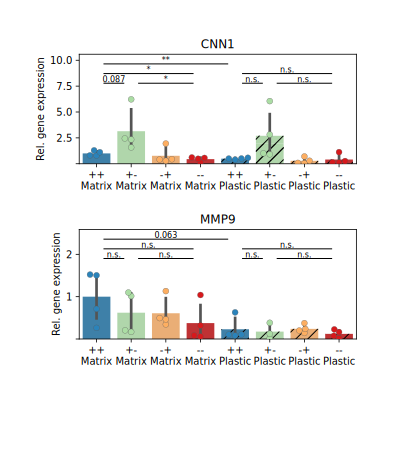
\includegraphics{Abbildung/qPCR.pdf}

    	\begin{minipage}{\captionwidth}
    		\caption[CNN_qPCR]{\uzlemph{Relative Expression of \ac{cnn1} and \ac{mmp9} in \acp{haosmc}} \newline qPCR analysis for expression of contractile marker \ac{cnn1} (top) and synthetic marker \ac{mmp9} (bottom) in \acp{haosmc} differentiated with different combinations of cytokines:
            \textbf{++:} four days with \ac{tgf} followed by two days with \ac{il1} and \ac{pdgf};
            \textbf{+–:} four days with \ac{tgf} followed by two days without stimulation;
            \textbf{–+:} four days without stimulation followed by two days with \ac{il1} and \ac{pdgf};
            \textbf{––:} six days without stimulation.
            All four conditions were tested on two different surfaces (plastic vs. \ac{col1} matrix). Expression levels are in relation to expression of housekeeping gene \ac{gapdh}. Statistical analysis for (n\,=\,4) biological repeats was performed using student's T-test: $*: p < 0.05; **: p < 0.01$}
    		\label{fig:qPCR_result}
    	\end{minipage}
    \end{figure}

    To confirm that the \acp{haosmc} first adopt a contractile phenotype and to track further differentiation after stimulation with \ac{pdgf}, the \ac{mRNA} levels of the marker genes \ac{cnn1} and \ac{mmp9} were determined using \ac{qpcr}. \ac{cnn1} serves as a contractile marker and \ac{mmp9} as a marker for a synthetic phenotype. For better comparability, \ac{mRNA} levels were normalized with the expression of the housekeeping gene \ac{gapdh}.\\
    Figure \ref{fig:qPCR_result} (top panel) illustrates that stimulation of \acp{haosmc} cultivated on a \ac{col1} matrix with \ac{tgf} causes a significant increase in \ac{cnn1} expression (+– vs. – –). After further stimulation with \ac{pdgf} and \ac{il1}, while not significant, \ac{cnn1} expression declines again (+– vs. ++) but is still significantly higher than in \acp{haosmc}, which were not stimulated (– – vs. ++). A similar trend is noticeble for \acp{haosmc} cultivated on plastic. However, this effect did not reach significance after four biological repeats. Additionally, stimulation of \acp{haosmc} on plastic with \ac{tgf}, followed by stimulation with \ac{pdgf} and \ac{il1}, yields a significantly lower expression of \ac{cnn1} (++ Matrix vs. ++ Plastic).\\
    As seen in the bottom panel of figure \ref{fig:qPCR_result}, no statistically significant trends can be observed after four biological repeats for the expression of \ac{mmp9}. Still, the average expression of \ac{mmp9} seems to increase on \ac{col1} matrix compared to plastic for all conditions. The most noticeable difference being between \acp{haosmc} treated first with \ac{tgf} as well as with \ac{pdgf} and \ac{il1} (++ Matrix vs. ++ Plastic, p\,=\,0.063).

    \pagebreak
    \subsection{Energy profile}
    \label{subsec:energy}
    In addition to the expression of \ac{cnn1} and \ac{mmp9}, the energy profiles of \acp{haosmc} were assessed via Seahorse Assay. It is important to note that the assay was carried out on plastic because the \ac{col1} matrix does not fit into the confined compartment created by the piston to record the \ac{ocr} and \ac{ecar}. Furthermore, only two biological repeats were evaluated because it became clear that all other experiments would be carried out on a \ac{col1} matrix. Therefore all the following considerations should take these decisions and limitations into account.

    \begin{figure}[h!]
    \capstart
        \centering
        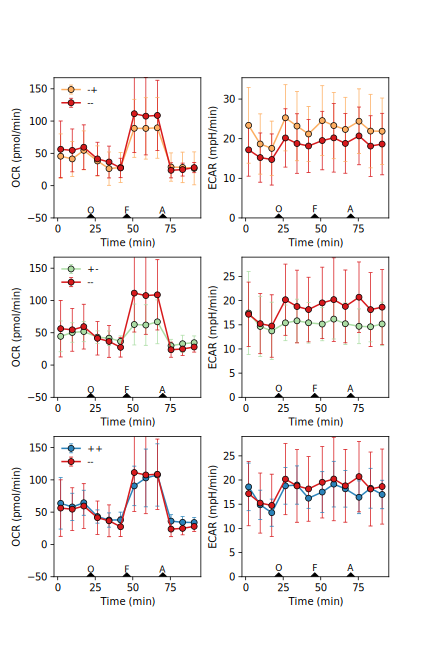
\includegraphics{Abbildung/Seahorse_tracks.pdf}

        \begin{minipage}{\captionwidth}
            \caption[seahorse_tracks]{\uzlemph{\ac{ocr} and \ac{ecar} of \acp{haosmc}} \newline Seahorse assay for \acp{haosmc} differentiated with different combinations of cytokines.
            \textbf{++:} four days with \ac{tgf} followed by two days with \ac{il1} and \ac{pdgf};
            \textbf{+–:} four days with \ac{tgf} followed by two days without stimulation;
            \textbf{–+:} four days without stimulation followed by two days with \ac{il1} and \ac{pdgf};
            \textbf{––:} six days without stimulation.
            \ac{ocr} and \ac{ecar} are shown for –+ (top), +– (middle) and ++ (bottom) compared to ––. Injection times for toxins (O: Oligomycin; F: FCCP; A: Antimycin A) are marked as triangles. All tracks were recorded for cells cultivated on plastic. Shown datapoints are the average of (n\,=\,2) biological repeats.
            }
            \label{fig:seahorse_tracks}
        \end{minipage}
    \end{figure}

    The readout parameters of the Seahorse assay are the \ac{ocr} as a representation of mitochondrial activity and the \ac{ecar}, representing the glycolytic activity of the cells. \ac{ocr} and \ac{ecar} for \acp{haosmc} are displayed in figure \ref{fig:seahorse_tracks}. All cells show characteristic changes in \ac{ocr} after the addition of toxins impacting the respiratory chain (compare to figure \ref{fig:seahorse_basics} B). After inhibition of the \ac{atp} synthase with Oligomycin, the basal \ac{ocr} drops, revealing the proportion of the \ac{ocr} required for \ac{atp} production. Subsequently, the addition of \ac{fccp} decouples the respiratory chain, destroying the proton gradient over the mitochondrial membrane. As a result, the cells reach their maximal respiratory capacity. Finally, the inhibition of coenzyme Q-cytochrome c reductase (complex III) with Antimycin A stops all mitochondrial respiratory activity.\\
    The \ac{ecar} shows a mild increase for all conditions after adding Oligionmycin, most likely because the cells compensate for the loss of mitochondrial \ac{atp} production via increased glycolysis.

    \begin{figure}[h!]
    \capstart
        \centering
    	\includegraphics{Abbildung/Seahorse_summary_merged.pdf}

    	\begin{minipage}{\captionwidth}
    		\caption[energy_profile]{\uzlemph{Energy profile of \acp{haosmc}} \newline Seahorse assay for \acp{haosmc} differentiated with different combinations of cytokines as described in figure \ref{fig:seahorse_tracks}.
            (\textbf{A}) Initial \ac{ocr} and \ac{ecar} of the four tested conditions. (\textbf{B}) Characteristics of the respiratory chain calculated from the tracks shown in figure \ref{fig:seahorse_tracks} as described in section \ref{sec:seahorse}. Statistical analysis for (n\,=\,2) biological repeats was performed using Welsh's T-test: $*: p < 0.05; **: p < 0.01, ; ***: p < 0.001$}
    		\label{fig:energy_profile}
    	\end{minipage}
    \end{figure}

    \pagebreak
    Looking at the energy profile, which describes the basal state of the differentiated cells, \ac{ocr} and \ac{ecar} are quite similar for the conditions ++, +–, and ––. The only outlier showing a higher \ac{ecar} are \acp{haosmc} only stimulated with only \ac{il1} and \ac{pdgf} (–+) (fig. \ref{fig:energy_profile}, A). More pronounced differences can be observed when examining the characteristics of the respiratory chain. Stimulation with only \ac{tgf} causes a significant decrease in basal respiration, \ac{atp} production, maximal respiration, and spare capacity (figure \ref{fig:energy_profile} B). Further stimulation with \ac{il1} and \ac{pdgf} then causes a significant increase of these parameters to similar levels as in initially dedifferentiated \acp{haosmc} (figure \ref{fig:energy_profile} B).

\section{Evaluation of oxidative Stress}
\label{sec:oxStress}
Finally, it was evaluated if further stimulation with \ac{pdgf} would stimulate the cells to generate \ac{ros} to the extent that can not be compensated by the \ac{ros} defense and lead to oxidative stress.

    \subsection{PDGF-BB boost of dedifferentiated HAoSMCs}

    \begin{figure}[h!]
    \capstart
        \centering
    	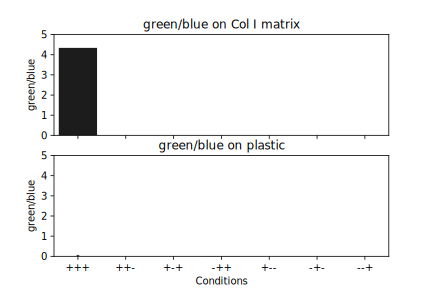
\includegraphics{Abbildung/CellROX_initial_cond.pdf}

    	\begin{minipage}{\captionwidth}
    		\caption[repeat_Lisa]{\uzlemph{Boost with \ac{pdgf} induces the generation of \ac{ros}.} \newline CellROX\texttrademark~assay for \acp{haosmc} differentiated with different combinations of cytokines: four days with \ac{tgf}; followed by two days with \ac{il1} and \ac{pdgf}; followed by 2\,h boost with 200\,ng/mL \ac{pdgf}. Differentiation and assay carried out on \ac{col1} matrix (top) or plastic (bottom). The shown signal was calculated according to section \ref{subsec:cellrox_data_processing} as the CellROX\texttrademark~Green signal, normalized by Hoechst 33342 signal. No statistical analysis for (n\,=\,1) biological repeats was performed. }
    		\label{fig:cellrox_8con}
    	\end{minipage}
    \end{figure}

    At first, an experiment already done in the group was validated. Stimulating the four tested combinations for 2 additional hours with 200\,ng/mL \ac{pdgf} in \ac{hbss}. As displayed in figure \ref{fig:cellrox_8con}, only stimulation for four days with \ac{tgf}, followed by two days with \ac{il1} and \ac{pdgf}, followed by a 2\,h boost with \ac{pdgf}, triggered noticeable \ac{ros} generation for cells cultivated on \ac{col1} matrix. No generation of \ac{ros} was detectable for \acp{haosmc} cultivated without the \ac{col1} matrix.

    \subsection{Characterization of the CellROX\texttrademark~Assay}
    \begin{figure}[h!]
    \capstart
        \centering
    	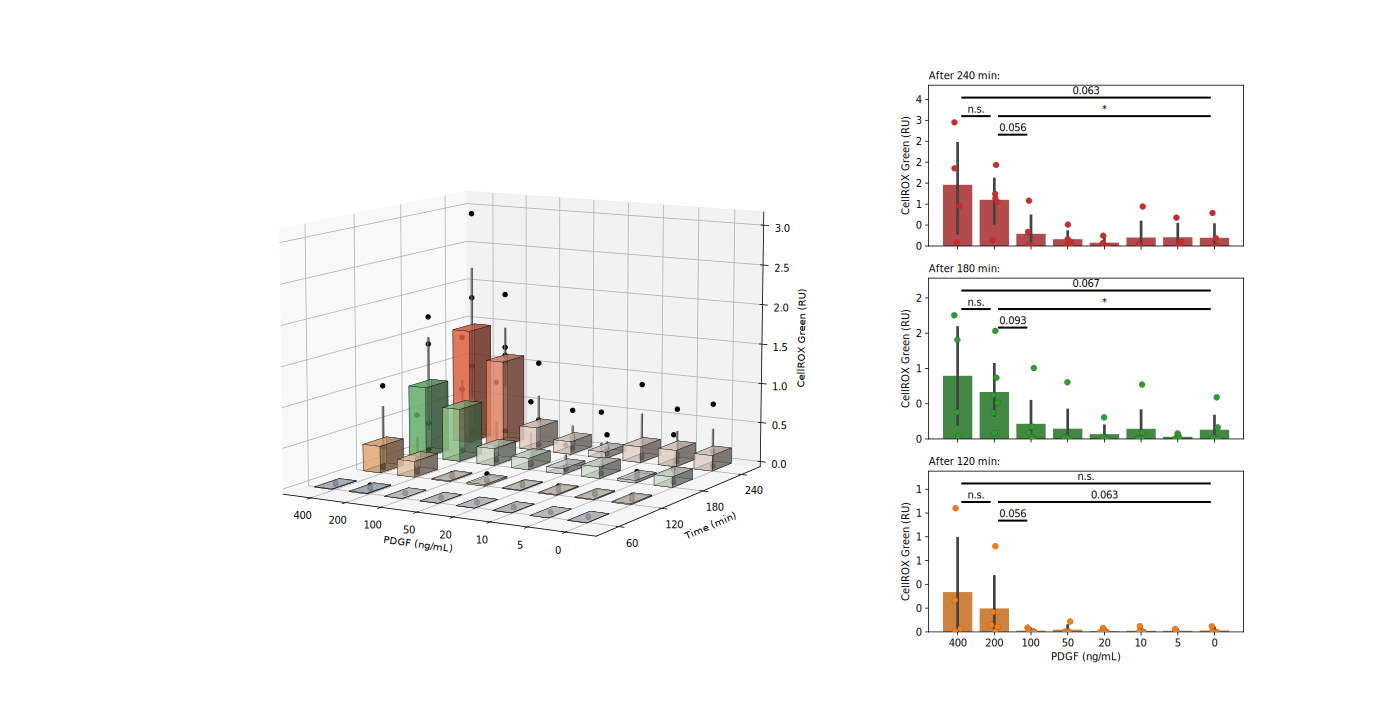
\includegraphics{Abbildung/CellROX_titration_no_norm.pdf}

    	\begin{minipage}{\captionwidth}
    		\caption[cellROX_titration]{\uzlemph{\ac{pdgf} boost titration} \newline
            CellROX\texttrademark~assay for \acp{haosmc} differentiated with different combinations of cytokines: four days with \ac{tgf}; followed by two days with \ac{il1} and \ac{pdgf}; followed by 4\,h boost with 0\,-\,400\,ng/mL \ac{pdgf}. Differentiation and assay carried out on \ac{col1} matrix.
            (\textbf{A}) 3D visualization: CellROX\texttrademark~Green signal as a function of \ac{pdgf} concentration during the boost as well as incubation time.
            (\textbf{B}) 2D visualization: CellROX\texttrademark~Green signal as a function of \ac{pdgf} concentration after 120 min, 180 min and 240\,min.
            The shown signal was calculated according to section \ref{subsec:cellrox_data_processing} as the CellROX\texttrademark~Green signal, normalized by Hoechst 33342 signal. Statistical analysis for (n\,=\,6) biological repeats was performed using Mann-Whitney U test: $*: p < 0.05$.}
    		\label{fig:cellROX_titration}
    	\end{minipage}
    \end{figure}

    To get a better understanding of the assay and its limits, a titration was carried out. For this, \acp{haosmc} stimulated for four days with 5\,ng/mL \ac{tgf} as well as two days with 10\,ng/mL \ac{il1} and 10\,ng/mL  \ac{pdgf}, were boosted with different concentrations of \ac{pdgf} (0\,-\,400\,ng/mL). Signal was detected after 60, 120, 180, and\,240 min in \ac{hbss} (figure \ref{fig:cell_rox_cells}). As seen in figure \ref{fig:cellROX_titration}, the CellROX\texttrademark~Green signal is negligible after 60\,min and then increases with elongated boost times. Moreover, CellROX\texttrademark~Green signal stays negligible for boost concentrations < 100\,ng/mL \ac{pdgf}. After 180 and 240\,min (figure \ref{fig:cellROX_titration} B top and middle), CellROX\texttrademark~Green signal is significantly increased for boost with 200\,ng/mL \ac{pdgf} compared to no boost (0\,ng/mL \ac{pdgf}). While the signal in wells boosted with 400\,ng/mL \ac{pdgf} was, on average higher than the signal after boost with 200\,ng/mL \ac{pdgf}, this increase was not reproducible. On the one hand, the signal was extremely high. On the other hand, the other two repeats, it collapsed.

    \begin{figure}[h!]
    \capstart
        \centering
    	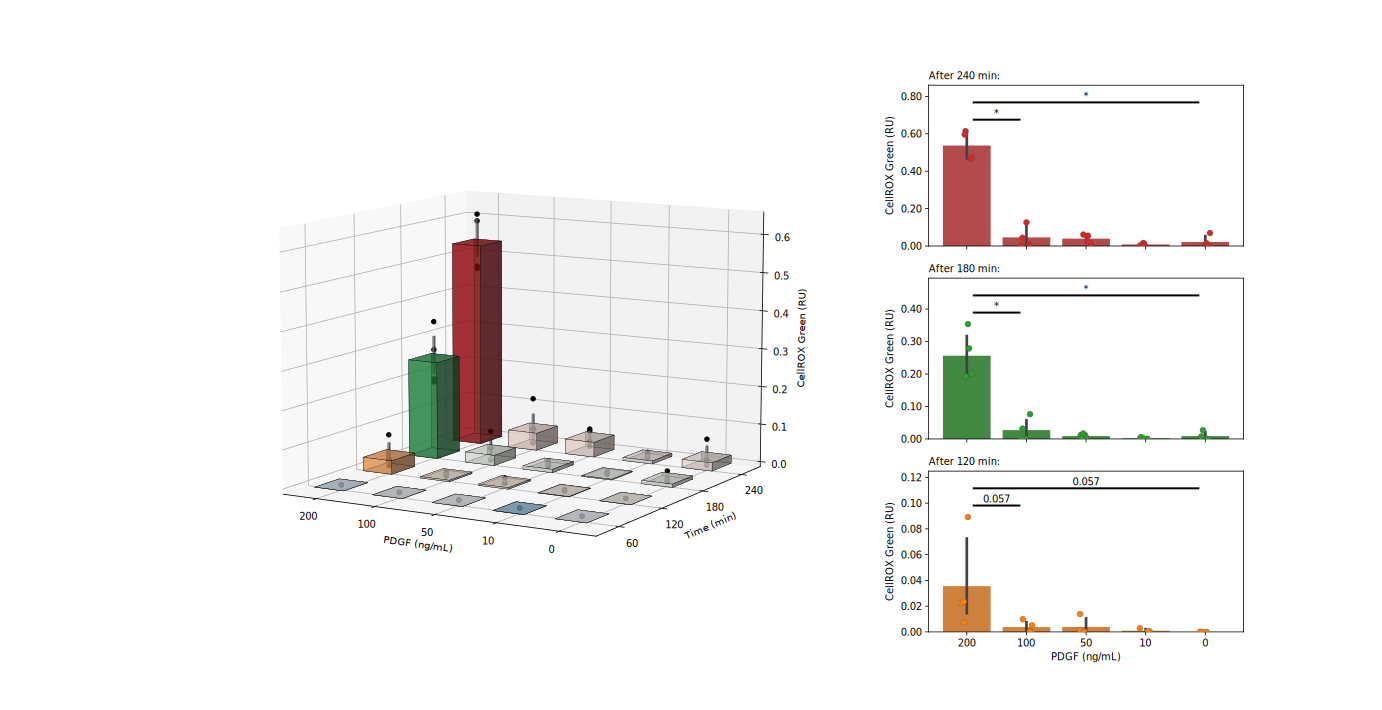
\includegraphics{Abbildung/CellROX_titration_norm.pdf}
    	\begin{minipage}{\captionwidth}
    		\caption[cellROX_titration_norm]{\uzlemph{\ac{pdgf} boost titration - normalized} \newline
            CellROX\texttrademark~assay for \acp{haosmc} differentiated with different combinations of cytokines: four days with \ac{tgf}; followed by two days with \ac{il1} and \ac{pdgf}; follwoed by 4\,h boost with 0\,-\,200\,ng/mL \ac{pdgf}. Differentiation and assay carried out on \ac{col1} matrix.
            (\textbf{A}) 3D visualization: CellROX\texttrademark~green signal as a function of \ac{pdgf} concnentration during the boost as well as incubation time.
            (\textbf{B}) 2D visualization: CellROX\texttrademark~green signal as a function of \ac{pdgf} concnentration after 120\,min, 180\,min and 240\,min.
            Shown signal was calculated according to section \ref{subsec:cellrox_data_processing} as the CellROX\texttrademark~Green signal, normalized by Hoechst 33342 signal, further the signal was normalized via the total signal of the biological repeat. Statistical analysis for (n\,=\,4) biological repeats was performed using Mann-Whitney U test: $*: p < 0.05$. Note that not every biological repeat covered \textit{all} \ac{pdgf} concentration.}
    		\label{fig:cellROX_titration_norm}
    	\end{minipage}
    \end{figure}

    Overall, the trend of greatly increased CellROX\texttrademark~signal for a boost with 100 or 200\,ng/mL \ac{pdgf} was consistent within biological repeats; however, the variance between repeats was almost as high as the differences between the conditions. To account for this large variation between biological repeats, the assay was reevaluated by the selection of shared conditions among the biological repeats normalized to the cumulative intensity of all conditions of the biological repeat (see figure \ref{fig:cellROX_titration_norm}). This step compensates for differences between biological repeats. The interpretation of the results remains unaffected by normalization: CellROX\texttrademark~Green signal after 180 and 240\,min is significantly higher for cells boosted with 200\,ng/mL \ac{pdgf} than cells that were not boosted (0\,ng/mL \ac{pdgf}).

    \subsection{Rescue of ROS production using NAC}
        \begin{figure}[h!]
    \capstart
        \centering
    	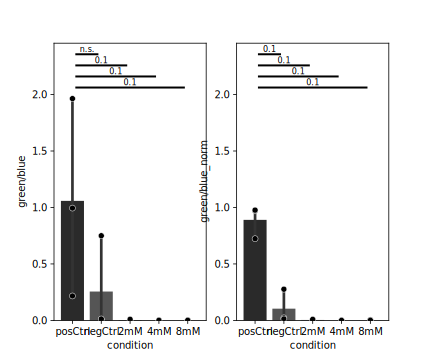
\includegraphics{Abbildung/NAC_quench.pdf}

    	\begin{minipage}{\captionwidth}
    		\caption[NAC quench]{\uzlemph{\ac{ros} generation due to \ac{pdgf} boost can be rescued with \ac{nac}} \newline
            CellROX\texttrademark~assay for \acp{haosmc} differentiated with different combinations of cytokines: four days with \ac{tgf}; followed by two days with \ac{il1} and \ac{pdgf}; followed by 3\,h boost with 200\,ng/mL \ac{pdgf}. Differentiation and assay carried out on \ac{col1} matrix. Cells were treated with 2, 4, or 8\,mM of \ac{nac} 2\,h before the assay.
            Shown signal was calculated according to section \ref{subsec:cellrox_data_processing} as the CellROX\texttrademark~Green signal, normalized by Hoechst 33342 signal (\textbf{A}), further the signal was normalized via the total signal of the biological repeat (\textbf{B}). Statistical analysis for (n\,=\,3) biological repeats was performed using Mann-Whitney U test: $*: p < 0.05$.
            pos Ctrl: not treated with \ac{nac}, negCtrl: no boost with \ac{pdgf}}
    		\label{fig:NAC_quench}
    	\end{minipage}
    \end{figure}

Finally, a rescue experiment was performed to verify that the observed signal in the CellROX\texttrademark~assay was due to the generation of \ac{ros}. \ac{ros} generation was quenched by adding 2,\,4,\,or 8\,mM of \ac{nac}. Indeed, a clear trend can be observed: \acp{haosmc} treated with \ac{nac} showed no signal. However, this trend remained statistically insignificant for triplicates.\\
It is noteworthy that the signal only builds up over 15\,-\,20\,min under the microscope after the cells were taken out of the incubator. This observation indicates that the generation of \ac{ros} might not be exclusively triggered by \ac{pdgf} boost. However, it could also require additional contributors like the loss of the optimized atmosphere of 37°C and 5\,\% \ac{co2} in the incubator. This fact might not have surfaced during the titration assay because cells were taken out of the incubator after one hour to image them for the first time.

\section{Database and GWAS Navigator}

    \subsection{Curation of Data}

    \begin{table}[h!]
    \capstart
    \centering
    \begin{minipage}{\captionwidth}
        \caption[db tables]{\uzlemph{List of database tables}\newline
    List of all the datasets and corresponding tables which were funneled into the database. For primary keys, foreign keys as well as fields on which an idex exists, please consulte figure \ref{fig:db_er}. The size of the tables (and accompanying indices) is indicated by the number of databank pages that are reserved for the data, each page fitting 4096 bytes.}
        \label{tab:db_tables}
    \end{minipage}
        \begin{tabular}{l|l|r}
        Data                                       & Tables                             & Page count\newline (including indices)                                                                      \\ \hline
        \multirow{3}{*}{GWAS Summary stats}        & variation                          & 418,318                                                                                              \\
                                                   & gwas\_meta\_cad                    & 867,025                                                                                              \\
                                                   & identified\_proxy\_SNPs\_tbl       & 4                                                                                                   \\ \hline
        \multirow{2}{*}{HGNC gene list}            & hgnc\_all\_symbols\_tbl            & 826                                                                                                 \\
                                                   & hgnc\_approved\_symbols\_tbl       & 592                                                                                                 \\ \hline
        \multirow{3}{*}{Linked SNPs}               & linked\_SNPs\_tbl                  & 8,819                                                                                                \\
                                                   & population\_tbl                    & 1                                                                                                   \\
                                                   & consequence\_tbl                   & 1                                                                                                   \\ \hline
        \multirow{2}{*}{Ensembl Genome Annotation} & ensembl\_genelist\_tbl             & 613                                                                                                 \\
                                                   & ensembl\_genelist\_biotypes\_tbl   & 1                                                                                                   \\ \hline
        \multirow{2}{*}{Ensembl Regulatory Build}  & ensembl\_reg\_build\_tbl           & 8,778                                                                                                \\
                                                   & ensembl\_reg\_build\_features\_tbl & 1                                                                                                   \\ \hline
        TSS                                        & tss\_tbl                           & 481                                                                                                 \\ \hline
        Open Target Genetics Scores                & opentarget\_l2g\_tbl               & 40,984                                                                                               \\ \hline
        \multirow{2}{*}{GWAS catalog}              & gwascatalog\_associations\_tbl     & 10,569                                                                                               \\
                                                   & gwascatalog\_studies\_tbl          & 326                                                                                                 \\ \hline
        \multirow{2}{*}{TADs}                      & tad\_tbl                           & 902                                                                                                 \\
                                                   & tad\_sample\_tbl                   & 1                                                                                                   \\ \hline
        \multirow{2}{*}{scATAC seq textcite\{\}}   & clint\_miller\_tbl                 & 12,370                                                                                               \\
                                                   & clint\_miller\_biotypes\_tbl       & 1                                                                                                   \\ \hline
        \multirow{2}{*}{scATAC seq CATlas}         & catlas\_tbl                        & 308,574                                                                                              \\
                                                   & catlas\_biotypes\_tbl              & 3                                                                                                   \\ \hline
        \multirow{4}{*}{ABC model}                 & abc\_tbl                           & 153,920                                                                                              \\
                                                   & abc\_targetgenes\_tbl              & 84                                                                                                  \\
                                                   & abc\_celltypes\_tbl                & 3                                                                                                   \\
                                                   & abc\_classes\_tbl                  & 1                                                                                                   \\ \hline
        \multirow{2}{*}{ENCODE cCREs}              & ENCODE\_CCRE                       & 4,451,476                                                                                             \\
                                                   & ENCODE\_CCRE\_META                 & 107                                                                                                 \\ \hline
        total                                      & -                                  & 6,284,781 ($\approx$ 25.75 GB)
        \end{tabular}
    \end{table}

    The first step toward visualization of \ac{gwas} summary statistics was curating relevant complementary data. Datasets from diverse data sources were downloaded and funneled into an SQLite3 database as described in section \ref{sec:database}. A \ac{sql} database is a two-dimensional relational database that allows easy and fast access to the data for visualization purposes. The data types and their applications are briefly described in section \ref{sec:bioinformatics}. All database tables and their sizes are summarized in table \ref{tab:db_tables}. The relationships between the tables and fields serving as a primary key, foreign, or fields on which an index exists are summarised in the database's \ac{er} diagram in figure \ref{fig:db_er}.

    \begin{figure}[h!]
    \capstart
        \centering
        \includegraphics{Abbildung/db-schema.pdf}

        \begin{minipage}{\captionwidth}
            \caption[database]{\uzlemph{Entity-Relationship diagram of the database}\newline
            Fields and relationships of the tables listed in table \ref{tab:db_tables}. On spelled out columns an index exists or they are primary or forgein keys. The diagram was generated via SchemaSpy.}
            \label{fig:db_er}
        \end{minipage}
    \end{figure}

    \begin{figure}[H]
        \vspace*{-0.5cm}
        \capstart
        \centering
        \includegraphics{Abbildung/GWAS_navigator_screenshot.pdf}

        \begin{minipage}{\captionwidth}
            \caption[database]{\uzlemph{The \ac{gwas} Navigator}\newline
            General content of the \aca{gwas} Navigator. The tool contains a manhattan plot with \ac{gwas} summary statistics, containing an additional annotation for variants that are in \ac{ld} with the variant central to the analysis. Further variants identified as proxy variants for other phenotypes are included. Finally, the data are aligned with genomic elements such as genes, regulatory elements, \ac{sc}\ac{atac} data as well as the \ac{abc} model. More details can be assessed by a hover effect as shown in figure \ref{fig:GWAS_navigator_hover}.}
            \label{fig:navigator}
        \end{minipage}
    \end{figure}

    \subsection{Visualization}
    \label{subsec:result_vis}
    Implementing the initially intended use case for the data, a visualization tool for \ac{gwas} summary statistics was built according to section \ref{sec:gwas_vis}. As shown in figure \ref{fig:navigator}, the \aca{gwas} Navigator consists of a separate search bar with a field to specifically search for variants by their rsID and a field that allows searching for genes by their symbol. If the searched gene is associated with one of the proxy variants in \textcite{aragamDiscoverySystematicCharacterization2021}, the tool returns a list of these variants. Else the tool returns the most significant variant in the proximity of the searched gene. After a variant is chosen, the tool displays the \ac{gwas} summary statistics in a 500 kb window centered around the selected variant to the output panel. \ac{gwas} summary statistics are visualized as a zoomed-in Manhatten plot, showing the position of a variant on \ac{hg38} on the x-axis and its p-value on the y-axis. $r^2$ values of variants in \ac{ld} are color-coded. In addition, the most severe consequence for all linked variants predicted by \ac{vep} is indicated by the type of glyph. The \ac{maf} and effect size (\beta) are included in the hover overlay (figure \ref{fig:GWAS_navigator_hover} A). Below this plot, variant trait associations from the \ac{gwas} catalog are indicated for variants that are in \ac{ld} with the variant central to the analysis (figure \ref{fig:GWAS_navigator_hover} B). Furthermore, the region is aligned with protein-coding genes, \acp{lncRNA} and \acp{miRNA} annotated in Ensembl. The names of genes that are associated with the variant of interest (open target genetics \ac{l2g} score > 0.3) are labeled in red. In addition, regulatory elements from the Ensembl regulatory build are displayed. Finally, sc\ac{atac} data and enhancers-promotor links from the \ac{abc} model were aligned, automatically hiding tracks with no elements in the visualized region.\\
    The \aca{gwas} Navigator also has a settings tab where individual tracks can be hidden.

    \begin{figure}[h!]
    \capstart
        \centering
        \includegraphics{Abbildung/GWAS_navigator_hover.pdf}

        \begin{minipage}{\captionwidth}
            \caption[database]{\uzlemph{The \ac{gwas} Navigator - hovereffect}\newline
            Exemplary hover effects for features displayed in the \aca{gwas} Navigator. (\textbf{A}) Hover for variants in the manhattan plot. (\textbf{B}) Hover for variant phenotype associations. (\textbf{C}) Hover for cell type specific enhancers in the \ac{abc} model.}
            \label{fig:GWAS_navigator_hover}
        \end{minipage}
    \end{figure}

\section{Enrichment analysis}
\label{sec:result_enrichment}
The only data not displayed in the plot are ENCODE \acp{cCRE} subjected to an enrichment analysis. The annotated biosamples are checked for significant enrichment of \acp{cCRE} that overlap with proxy \acp{snp} identified by the ARDIoGRAMplusC4D Consortium \cite{aragamDiscoverySystematicCharacterization2021} or variants in \ac{ld} with these ($r^2 > 0.6$). For more details, please refer to section \ref{sec:enrichment}.

\begin{figure}[h!]
\capstart
    \centering
	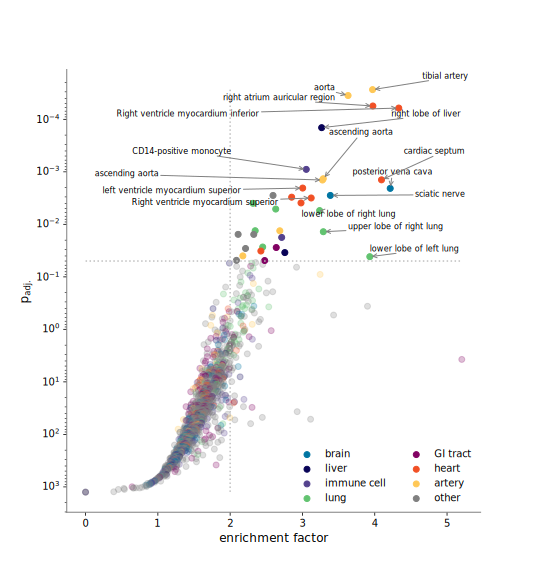
\includegraphics{Abbildung/enrichment_scatter.pdf}

	\begin{minipage}{\captionwidth}
		\caption[enrichemtn]{\uzlemph{Enrichment analysis for overlap of \ac{cad} \ac{gwas} proxy variants with tissue specific \acp{cCRE}} \newline p-values and enrichment factors for the overlap of CARDIoGRAMplusC4D proxy variants (and variants in \ac{ld}) with tissue specific \acp{cCRE}. For details please refer to section \ref{sec:enrichment}.}
		\label{fig:enrichment_scatter}
	\end{minipage}
\end{figure}

As seen in figure \ref{fig:enrichment}, statistically significant enrichment ($p_{adj.}<0.05$) was observed for 34 biosamples (table \ref{tab:enriched_tissues_all}). Using the biosample annotations from Cellosaurus, these biosamples were assigned to their tissue of origin. The most prominent groups of origin tissues are the heart (8), the lungs (7), and arteries (6), as summarized in table \ref{tab:enriched_tissues}. Other tissues included the liver, the \ac{gi} tract, the brain, and immune cells (CD14\textsuperscript{+} monocytes).


\begin{table}[h!]
\capstart
\centering
\begin{minipage}{\captionwidth}
    \caption[enriched tissues]{\uzlemph{Tissues found in the enrichment analysis} \newline Tissues of biosamples which show statitically significant overlap between CARDIoGRAMplusC4D Consortium proxy variants (and variants in \ac{ld}) and \acp{cCRE}.}
    \label{tab:enriched_tissues}
\end{minipage}
\begin{tabular}{|c|c|}
    \hline
    tissue      & count in significant biosamples \\ \hline
    heart       & 8                               \\
    lung        & 7                               \\
    artery      & 6                               \\
    liver       & 2                               \\
    GI tract    & 2                               \\
    brain       & 2                               \\
    immune cell & 2                               \\
    other       & 5                               \\ \hline
    total       & 34                              \\ \hline
    \end{tabular}
\end{table}


\begin{landscape}
\begin{table}[h!]
\vspace*{-1cm}
\capstart
\centering
\begin{minipage}{\captionwidth}
    \caption[enriched samples]{\uzlemph{List of all biosamples that show significant enrichment}}
    \label{tab:enriched_tissues_all}
\end{minipage}
    \begin{tabular}{r|r|r|r|r|r|r|l|l|l}
    nt & mt     & n   & m       & p        & p\_adj   & ef & biosample\_term\_name                                  & cellosaurus\_attr\_2 & cellosaurus\_attr\_3 \\ \hline
    23 & 60010  & 165 & 1709065 & 2.16e-08 & 2.72e-05 & 3.96              & tibial artery                                          & artery               & artery               \\
    25 & 71318  & 165 & 1709065 & 2.80e-08 & 3.52e-05 & 3.63              & aorta                                                  & aorta                & artery               \\
    22 & 57342  & 165 & 1709065 & 4.43e-08 & 5.57e-05 & 3.97              & right atrium auricular region                          & cardiac atrium       & heart                \\
    20 & 47820  & 165 & 1709065 & 4.85e-08 & 6.10e-05 & 4.33              & Right ventricle myocardium inferior                    & myocard              & heart                \\
    26 & 82463  & 165 & 1709065 & 1.14e-07 & 1.44e-04 & 3.26              & right lobe of liver                                    & liver                & liver                \\
    25 & 84828  & 165 & 1709065 & 7.14e-07 & 8.97e-03 & 3.05              & CD14-positive monocyte                                 & monocytes            & immune cell          \\
    22 & 69308  & 165 & 1709065 & 1.07e-06 & 1.35e-03 & 3.28              & ascending aorta                                        & aorta                & artery               \\
    17 & 43017  & 165 & 1709065 & 1.13e-06 & 1.42e-03 & 4.09              & cardiac septum                                         & cardiac septum       & heart                \\
    22 & 69542  & 165 & 1709065 & 1.13e-06 & 1.43e-03 & 3.27              & ascending aorta                                        & aorta                & artery               \\
    24 & 82774  & 165 & 1709065 & 1.62e-06 & 2.03e-03 & 3.00              & left ventricle myocardium superior                     & myocard              & heart                \\
    16 & 39330  & 165 & 1709065 & 1.64e-06 & 2.06e-03 & 4.21              & posterior vena cava                                    & neuronal cell        & brain                \\
    20 & 61185  & 165 & 1709065 & 2.23e-06 & 2.81e-03 & 3.38              & sciatic nerve                                          & neuronal cell        & brain                \\
    29 & 115843 & 165 & 1709065 & 2.24e-06 & 2.81e-03 & 2.59              & \begin{tabular}[c]{@{}l@{}}dermis microvascular lymphatic vessel \\ endothelial cell\end{tabular} & endothelial cell     & lymphatic vessel     \\
    25 & 90831  & 165 & 1709065 & 2.41e-06 & 3.03e-03 & 2.85              & heart left ventricle                                   & heart left ventricle & heart                \\
    22 & 73021  & 165 & 1709065 & 2.50e-06 & 3.14e-03 & 3.12              & Right ventricle myocardium superior                    & myocard              & heart                \\
    23 & 79943  & 165 & 1709065 & 3.10e-06 & 3.90e-03 & 2.98              & left ventricle myocardium inferior                     & myocard              & heart                \\
    34 & 152031 & 165 & 1709065 & 3.16e-06 & 3.97e-03 & 2.31              & lung microvascular endothelial cell                    & endothelial cell     & lung                 \\
    27 & 106321 & 165 & 1709065 & 4.07e-06 & 5.11e-03 & 2.63              & right lung                                             & lung                 & lung                 \\
    20 & 63984  & 165 & 1709065 & 4.34e-06 & 5.46e-03 & 3.23              & lower lobe of right lung                               & lung                 & lung                 \\
    30 & 132446 & 165 & 1709065 & 1.05e-05 & 1.32e-02 & 2.34              & lung microvascular endothelial cell                    & endothelial cell     & lung                 \\
    24 & 92520  & 165 & 1709065 & 1.05e-05 & 1.32e-02 & 2.68              & dermis blood vessel endothelial cell                   & endothelial cell     & artery               \\
    18 & 56694  & 165 & 1709065 & 1.09e-05 & 1.38e-02 & 3.28              & upper lobe of right lung                               & lung                 & lung                 \\
    36 & 176705 & 165 & 1709065 & 1.23e-05 & 1.55e-02 & 2.11              & subcutaneous abdominal adipose tissue                  & adipocyte            & adipose tissue       \\
    30 & 133565 & 165 & 1709065 & 1.23e-05 & 1.55e-02 & 2.32              & ovary                                                  & ovary                & ovary                \\
    23 & 87812  & 165 & 1709065 & 1.41e-05 & 1.77e-02 & 2.71              & CD14-positive monocyte                                 & monocytes            & immune cell          \\
    26 & 109915 & 165 & 1709065 & 2.15e-05 & 2.70e-02 & 2.45              & left lung                                              & lung                 & lung                 \\
    23 & 90330  & 165 & 1709065 & 2.19e-05 & 2.76e-02 & 2.63              & left colon                                             & colon                & GI tract             \\
    31 & 145102 & 165 & 1709065 & 2.29e-05 & 2.88e-02 & 2.21              & endothelial cell of umbilical vein                     & endothelial cell     & embyro               \\
    26 & 111050 & 165 & 1709065 & 2.56e-05 & 3.21e-02 & 2.42              & heart                                                  & heart                & heart                \\
    21 & 78914  & 165 & 1709065 & 2.74e-05 & 3.44e-02 & 2.75              & left lobe of liver                                     & liver                & liver                \\
    31 & 147590 & 165 & 1709065 & 3.17e-05 & 3.98e-02 & 2.17              & dermis blood vessel endothelial cell                   & endothelial cell     & artery               \\
    13 & 34248  & 165 & 1709065 & 3.28e-05 & 4.12e-02 & 3.93              & lower lobe of left lung                                & lung                 & lung                 \\
    33 & 163804 & 165 & 1709065 & 3.85e-05 & 4.84e-02 & 2.08              & kidney                                                 & kidney               & kidney               \\
    24 & 100336 & 165 & 1709065 & 3.88e-05 & 4.88e-02 & 2.47              & mucosa of gallbladder                                  & gallbladder          & GI tract
    \end{tabular}
\end{table}
\end{landscape}


%%%%%%%%%%%%%%%%%
%               %
%   Diskussion  %
%               %
%%%%%%%%%%%%%%%%%

\chapter{Discussion}
\section{PDGF-BB signaling induces a synthetic phenotype in HAoSMCs}
The crucial role of \acp{vsmc} in atherogenesis has been the subject of extensive research for the last few decades \cite{grootaertVascularSmoothMuscle2021, yapSixShadesVascular2021}. Traditionally it has been assumed that \acp{vsmc} adopt a protective role by stabilizing the atherosclerotic plaque. This model is rapidly evolving and starting to consider the existence of a diverse set of dedifferentiated phenotypes \cite{liuSmoothMuscleCell2019}. A central hub of the dedifferentiation process is an initial mesenchymal-like phenotype. This phenotype exhibits a proliferative phenotype and reduced expression of contractile markers \cite{yapSixShadesVascular2021}. This phenotype is thought to be initiated by the \ac{tf} \ac{klf4}, which induces the expression of mesenchymal markers such as \ac{sca1} \cite{yapSixShadesVascular2021}. Amongst other pathways, expression of \ac{klf4} can be induced by \ac{pdgf} signaling \cite{liuKruppellikeFactorAbrogates2005} via \ac{sp1} \cite{deatonSp1dependentActivationKLF42009}. Additionally, \ac{pdgf} suppresses the contractile phenotype by phosphorylation of \ac{elk-1} \cite{wangMyocardinTernaryComplex2004} as well as the expression of \ac{dock2} \cite{guoDedicatorCytokinesisNovel2015}. Both processes disrupt myocardin/\ac{srf} mediated expression of contractile genes. The mesenchymal-like phenotype is postulated as a precursor for other dedifferentiated \acp{vsmc} phenotypes \cite{yapSixShadesVascular2021}.\\
The contractile differentiated \acp{vsmc} phenotype is constantly maintained by myocardin/\ac{srf} signaling \cite{longMyocardinSufficientSmooth2008}, as well as external stimulation by the \ac{ecm} and cytokines such as \ac{tgf} \cite{davis-dusenberyDownregulationKruppellikeFactor42011}. \acp{haosmc} used in this thesis seem to have initially adopted a dedifferentiated phenotype, characterized by the loss of contractile marker \ac{cnn1} \cite{owensMolecularRegulationVascular2004} (figure \ref{fig:qPCR_result} top). When stimulated with \ac{tgf} for four days, \acp{haosmc} display increased expression of \ac{cnn1}. Additionally, this phenotype shows a significant decrease in  basal mitochondrial respiration, ATP production, and maximal respiration (figure \ref{fig:energy_profile} B). This trend is possibly an adaptation to the energetic needs of the contractile phenotype, which is considered quiescent \cite{dobnikarDiseaserelevantTranscriptionalSignatures2018}. Further simulation with \ac{pdgf} and \ac{il1} for two days yields a the decrease expression of \ac{cnn1}, on the verge of significance (p=0.087). Moreover, the energy metabolism changes again, characterized by a rebound of basal mitochondrial respiration, \ac{atp} production, and maximal respiration to similar levels as initially dedifferentiated VSMCs (figure \ref{fig:energy_profile} B).\\
Another important aspect of phenotypic transition and plaque development is the remodeling of the \ac{ecm} by \acp{mmp} \cite{johnsonMetalloproteinasesAtherosclerosis2017}.
Our experiments hint toward a possible increase of \ac{mmp9} expression for \acp{haosmc} cultivated on \ac{col1} matrix (figure \ref{fig:qPCR_result} bottom) after \ac{pdgf}-induced dedifferentiation. However, this trend remained not significant in four biological replicates (p = 0.063). \ac{mmp9} is an important component of atherosclerogenesis \cite{galisIncreasedExpressionMatrix1994} and a biomarker for advanced atherosclerotic lesions \cite{langleyExtracellularMatrixProteomics2017}. The fact that this trend is only observable for cells cultivated on \ac{col1} (figure \ref{fig:qPCR_result} bottom) underlines the bi-directionality of the \ac{ecm}-\ac{vsmc}-interactions and the complexity of \ac{vsmc} dedifferentiation.\\
Of course, the \ac{pdgf}-induced phenotype can not be grasped with only two markers and requires a more in-depth analysis, for example via \ac{rna}-sequencing.


\section{CellROX\texttrademark~Green is suitable for assessing ROS generation in HAoSMCs}
Evaluating the response to further stimulation with \ac{pdgf}, the CellROX\texttrademark~Assay confirmed a result previously observed in the group (unpublished). Stimulation of \acp{haosmc} cultivated on \ac{col1} matrix and treated for four days with \ac{tgf} and two days with \ac{pdgf} and \ac{il1} are susceptible to the generation of \ac{ros} by \ac{pdgf} boost (figure \ref{fig:cellrox_8con}).\\
Further evaluating the limits of the used assay, it is obvious that a threshold concentration of 200\,ng/ml \ac{pdgf} is required to induce a significant increase in signal over the negative control (0\,ng/mL) (figure \ref{fig:cellROX_titration}). In addition, it was observed that the signal intensity highly depends on the incubation time. While the trend for each biological repeat is clear, the variance between repeats is in a similar range. The assay is working reliably but could greatly benefit from retroactive normalization (figure \ref{fig:cellROX_titration_norm}) or further optimization of reproducibility - reducing the required amount of biological repeats. An alternative option for normalization could be provided by direct stimulation with \ac{h2o2} to be used as a reference. Finally, the robustness of the assay may be improved by the exploration of different CellROX\texttrademark~Green concentrations.\\
Finally, a recovery experiment was performed. Before and during the boost, cells were co-incubated with \ac{nac}. \ac{nac} is a popular and potent antioxidant used in cell culture experiments, and it likely acts by being metabolized into sulfane sulfur species that scavenge \ac{ros} in the mitochondria \cite{ezerinaNAcetylCysteineFunctions2018}. Cells treated with \ac{nac} showed only little to no CellROX\texttrademark~Green signal. Even though this trend remained not significant after three replicates, it supports the expectation that the observed signal is indeed due to the generation of \ac{ros} (figure \ref{fig:cellROX_titration_norm}).\\
Moreover, it needs to be evaluated if the used \ac{pdgf} concentration of 200\,ng/ml ($\widehat{=}$8.25\,nM) is physiologically relevant. Unfortunately, cytokine concentrations are usually assessed as plasma concentrations, and no \textit{in vivo} data exists for local concentrations during paracrine signaling. While the manufacturer describes the \ac{ec50} for \ac{pdgf}-induced proliferation of Balb/c 3T3 cells between 1.0\,-\,3.0\,ng/mL \cite{peprotecheclimitedRecombinantHumanPDGFBB2022}, higher concentrations have frequently been used in the literature. \textcite{gravesPlateletderivedGrowthFactor1996a} observed increased formation of \ac{camp} up to 10 nM ($\widehat{=}$240\,ng/mL) \ac{pdgf} when assessing the dose-response relationship between \ac{camp} formation after \ac{pdgf} stimulation of SMCs. \textcite{newmanMultipleCellTypes2021a} used 50\,ng/mL \ac{pdgf} for the differentiation of murine \acp{vsmc} in the context of atherosclerosis, and \textcite{bouziguesRegulationROSResponse2014a} identified 100\,ng/mL as a saturating concentration for the generation of \ac{h2o2} as a response to \ac{pdgf} signaling in \acp{vsmc}.\\
The next up-and-coming experiment would be the rescue experiment to confirm that the generation of \ac{ros} is indeed caused by \ac{pdgf} stimulation. Namely by the knockdown of the \ac{pdgfr}\beta. The same approach could be pursued to study downstream factors of \ac{pdgfr} signaling that are involved in the generation of \ac{ros}. An exemplary candidate would be the transcription factor \ac{stat1}, which upon deletion, reduces plaque formation during atherogenesis and is a required component of \ac{pdgf_simple}-signaling induced inflammation \cite{hePDGFRbetaSignallingRegulates2015}. In addition to its genomic function, \ac{stat1} can be imported into mitochondria, where it interacts with respiratory complexes and triggers the generation of \ac{ros} \cite{wangSTATROSCycleExtends2018} during hepatic apoptosis \cite{leeRoleSTAT1IRF12007} and \ac{ifn} induced cancer cell apoptosis \cite{wangSTATROSCycleExtends2018}.\\
Finally, it has to be addressed that during the recovery experiment with \ac{nac}, the CellROX\texttrademark~Green signal would occasionally only develops outside the controlled environment in the incubator. This suggests that the \ac{pdgf} is not the sole trigger of \ac{ros} generation. Repeating the experiment under better-controlled conditions would be a great option to follow up on this idea\\
We additionally tried to assess oxidative stress with an anti-8-oxoguanine antibody that detects 8-oxoguanine, a base modification often observed in the presence of \ac{ros} \cite{leon8OxoguanineAccumulationMitochondrial2016}. This attempt was not successful because the starvation of \acp{haosmc} for seven days in M231 supplemented with 1\,\%\,\ac{fbs} was sufficient to induce oxidative damage to the genome (figure \ref{fig:antibody}).


\section{The GWAS Navigator}
Like all primates, humans are extremely visual creatures. We have evolved specialized brain structures for processing visual stimuli \cite{kaasCurrentResearchOrganization2014}, granting us superior recognition of visual patterns \cite{mattsonSuperiorPatternProcessing2014}. Thus, making data visualization tools powerful and important resources for interactive data exploration and scientific communication.\\
The \aca{gwas} Navigator was developed to display CARDIoGRAMplusC4D Consortium \cite{aragamDiscoverySystematicCharacterization2021} summary statistics in a comprehensive and visually appealing format for medical researchers. In an iterative process, many possible implementation approaches were explored, finally resulting in the prototype presented in this thesis. At this point, the tool is built as a bokeh application (section \ref{sec:gwas_vis}) that dynamically fetches data from an SQLite database and renders it to the browser.\\
Databases are a structured data collection at the heart of data science. Databases provide many advantages over data stored in spreadsheets, such as access speed, maintainability, and multiuser access. They are designed to hold large data collections and provide secure and fast access by querying via specifically designed database engines. Relational databases, like SQLite, are the most popular way for flexibly representing data in tables comprising columns and rows. They are usually queried and manipulated with commands in \ac{sql}, an internally consistent, human-readable programming language. \cite{oraclecorporationWhatDatabase2022, oraclecorporationWhatRelationalDatabase2022} SQLite is a public domain database engine that generates cross-platform, single file databases and is the most used database engine worldwide \cite{thesqliteconsortiumSQLite2022}.\\
While certainly not the only option, bokeh fulfills all the basic requirements for the task. The package combines the elegant visualization resources for rendering data with \ac{html}, \ac{css}, and \ac{js} to the browser with the powerful data processing capabilities of python. All are bundled into one easy-to-learn ecosystem, providing a level of abstraction required for a prototype's construction. Additionally, the bokeh server makes the application easily deployable for potential use on a local network \cite{bokehdevelopmentteamBokehPythonLibrary2022}. \\
To summarize, the \aca{gwas} Navigator grants an overview of the genomic context of disease-associated genomic loci. The next step in its development should undoubtedly be the local deployment for the rest of the group. It provides basic functionality and the possibility to implement many additional features. Options range from basic improvements to usability in the formed tissue-specific annotations to the displayed tracks and the selection tool to the adoption of new datasets.


\section{Overlap of CAD associated variants with regulatory elements is enriched in heart, artery, and lung tissue}
In addition to providing the basis for the \aca{gwas} Navigator, the database also makes the data easily accessible for follow-up studies. The curated data are utilized in an initial postGWAS analysis, scanning for CARDIoGRAMplusC4D Consortium \cite{aragamDiscoverySystematicCharacterization2021} proxy variant enrichment in biosample-specific \acp{cCRE} via Fisher's exact test. This way identifying 34 biosamples (of 1257 tested) that show significant overrepresentation (figure \ref{fig:enrichment_scatter} and table \ref{tab:enriched_tissues}). After annotating these biosamples, over 40\,\% (14/34) of enriched biosamples stem from heart or artery tissue and are directly affected by atherosclerosis. An additional 20\,\% was annotated to stem from lung tissue, an observation in line with the frequently reported association between heart- and lung diseases \cite{carterAssociationCardiovascularDisease2019, hanPulmonaryDiseasesHeart2007}. The association of heart- and lung diseases prevails even after adjustment for shared risk factors such as tobacco usage or age. Additionally, \textcite{auyeungAssociationGeneticInstrumental2018} demonstrated via Mendelian randomization that greater \ac{fev1} decreases the risk of \ac{cad}. Still, the causality of this relationship remains unclear. While it is tempting to speculate that impaired lung function or systematic inflammation by \ac{copd} results in an elevated risk for cardiovascular diseases, such hypotheses are difficult to evaluate due to reverse causation \cite{nowakLungFunctionCoronary2018}. \ac{cad} might also be a risk factor for lung diseases, or both pathologies could share additional mutually relevant confounding factors. Similarly, the identification of lung tissue in our analysis might point toward the contribution of the lung during the development of \ac{cad} or a shared genomic predisposition of heart- and lung disease. Following up on systemic inflammation, the immune cells in which \acp{cCRE} enrich are CD14\textsuperscript{+} monocytes (table \ref{tab:enriched_tissues_all}), a cell type known for the secretion of proinflammatory cytokines during injury or inflammation \cite{kapellosHumanMonocyteSubsets2019}. Interestingly, CD14\textsuperscript{++}CD16\textsuperscript{+}CCR2\textsuperscript{+} and CD14\textsuperscript{++}CD16\textsuperscript{-}CCR2\textsuperscript{+} monocytes show significantly higher counts in patients with acute \ac{hf} over patients with stable \ac{hf} or \ac{cad} \cite{wrigleyCD14CD16Monocytes2013}.
\pagebreak
Finally, the same method and already collected data could be applied to check for the overlap of disease-associated variants with the enhancers identified as part of the \ac{abc} model. Consequently, based on the enhancer promotor connection, one may be able to identify potentially affected genes.


%%%%%%%%%%%%%%%%%
%               %
% Bibliographie %
%               %
%%%%%%%%%%%%%%%%%

\chapter*{Bibliography}
\addcontentsline{toc}{chapter}{Bibliography}
\markboth{Bibliography}{Bibliography}
\printbibliography[heading=none]

%%%%%%%%%%%%%%%%%
%               %
%  Abk. Verz.   %
%               %
%%%%%%%%%%%%%%%%%

\chapter*{Abbreviations and units}
\addcontentsline{toc}{chapter}{Abbreviations and units}
\markboth{Abbreviations and units}{Abbreviations and units}
\printacronyms[heading=section*, include=acronym, template=tabularray, name=Abbreviations]
\printacronyms[heading=section*, include=unit, template=tabularray, name=Units]

%%%%%%%%%%%%%%%%%
%               %
%  Supplement   %
%               %
%%%%%%%%%%%%%%%%%

\setcounter{chapter}{19}% Equivalent to "letter S"
\renewcommand{\thechapter}{\Alph{chapter}}
\chapter*{Supplement}
\setcounter{figure}{0}
\renewcommand{\thefigure}{S.\arabic{figure}}
\addcontentsline{toc}{chapter}{Supplement}
\markboth{Supplement}{Supplement}

\section{CellROX\texttrademark~assay}
\begin{figure}[H]
    \capstart
    \centering
    \includegraphics{Abbildung/cellrox_titration_wells_example.pdf}

    \begin{minipage}{\captionwidth}
        \caption[cell_rox_cells]{\uzlemph{Representative CellROX\texttrademark Green signal for \ac{pdgf} titration}\newline
        }
        \label{fig:cell_rox_cells}
    \end{minipage}
\end{figure}

\section{Evaluation of oxidative stress with an anti-8-oxoguanine antibody}
\subsection{Antibodies}
\begin{longtblr}[]{
    colspec = {X|X|X},
    rowhead = 1
}
    \textbf{Name}                            & \textbf{Species} & \textbf{Manufacturer}    \\ \hline
    Anti-8-Oxoguanine Antibody, clone 483.15 & mouse   & \SigmaA \\
    AF568 anti mouse                         & ?       & ?
\end{longtblr}

\subsection{Chemicals}
\begin{longtblr}[]{
    colspec = {X|X},
    rowhead = 1
}
    \textbf{Name} &  \textbf{Manufacturer} \\ \hline
    Acetone      & \Roth            \\
    \acs{dapi}          & \SigmaA            \\
    Methanol ($\geq$99\,\%)      & \Roth            \\
    Trition\textregistered X-100 & \Thermo
\end{longtblr}

In \ac{if} flourescently labeled antibodies are used to specifically target and label a molecule in a biological sample. An anti-8-oxoguanine antibody was used as a complementary approach to CellROX\texttrademark~assay. 8-oxoguanine is a common base lesion that is caused by the oxidation of guanine in the presence of \ac{ros} \cite{leon8OxoguanineAccumulationMitochondrial2016}.\\
For the assay, \acp{haosmc} differentiated according to section \ref{subsec:differentiation} on \ac{col1} matrix were washed with \ac{pbs} and boosted for 90\,min with 500\,mL \ac{M231} supplemented with 1\,\% \ac{fbs} and 200\,ng/mL \ac{pdgf}. After, the cells were fixated with 200\,µL methanol (1:1, -\,20\,°C) for 40\,min. The methanol:aceton was removed and cells were dried for 20\,min. For permeabilization, the cells were incubated with 250\,µL 0.2\,\% Triton\textregistered X-100, 1,\% BSA (in \ac{pbs}) for 30\,min. Further, unspecific binding sites were blocked with 250\,µL 3.5\,\% BSA (in \ac{pbs}) for 30\,min. Afterward, \acp{haosmc} were incubated with 500\,µL of the primary antibody (1:500 in \ac{pbs}) at 4\,°C over night. In the morning the cells incuabed with 500 µL AF555 anti mouse (1:1000 in \ac{pbs}) and nuclei were stained with \acf{dapi} (1:5000) for 1\,h.

\begin{figure}[H]
    \capstart
    \centering
    \includegraphics{Abbildung/8oxoG.pdf}

    \begin{minipage}{\captionwidth}
        \caption[antibody]{\uzlemph{Evaluation of oxidative stress with an anti-8-oxoguanine antibody}\newline
        }
        \label{fig:antibody}
    \end{minipage}
\end{figure}

Unfortunately, this approach was unsuccessful, because, as seen in figure \ref{fig:antibody}, starvation of \acp{haosmc} in \ac{M231} supplemented with 1\,\% \ac{fbs} was oxidation of guanine.

\end{document}
